\documentclass[refman]{scrartcl}
% ----------------------------------------------------------------------------------------------------------
% HEADER
% ----------------------------------------------------------------------------------------------------------

\usepackage[english]{babel}
\usepackage[utf8]{inputenc}

\usepackage{fancyhdr}
\usepackage{graphicx}
\usepackage[dvipsnames]{xcolor} 
\usepackage{epigraph}

\usepackage{amsmath}
\usepackage{amsthm}
\usepackage{amssymb}

\usepackage{listings}

\usepackage{titlesec}

\pagestyle{fancy}

\theoremstyle{definition}
\newtheorem{definition}{Definition}
\newtheorem{lemma}{Lemma}
\newtheorem{exmp}{Example}
\newtheorem{remark}{Remark}
\newtheorem{theorem}{Theorem}



\setcounter{secnumdepth}{4}

\titleformat{\paragraph}
{\normalfont\normalsize\bfseries}{\theparagraph}{1em}{}
\titlespacing*{\paragraph}
{0pt}{3.25ex plus 1ex minus .2ex}{1.5ex plus .2ex}

\begin{document}
%
% ----------------------------------------------------------------------------------------------------------
% TITLEPAGE & TABLE OF CONTENTS
% ----------------------------------------------------------------------------------------------------------
%
\begin{titlepage}
	\centering
	
\includegraphics[width=0.15\textwidth]{images/huberlin_logo}\par\vspace{1cm}
	{\scshape\LARGE Humboldt University of Berlin \par}
	\vspace{1cm}
	{\scshape\Large Einf{\"u}hrung in das wissenschaftliche Rechnen \par}
	\vspace{1.5cm}
	{\huge\bfseries Analysis of selected sorting Algorithms\par}
	\vspace{2cm}
	{\Large\itshape Christian Parpart \& Kei Thoma \par}
	\vfill

	\vfill

% Bottom of the page
	{\large \today\par}
\end{titlepage}

\tableofcontents
\newpage
%
% ----------------------------------------------------------------------------------------------------------
% CONTENTS
% ----------------------------------------------------------------------------------------------------------
%
% change section names later
\section{Introduction}
%
It is perhaps the most profound realization
\newpage
%
\section{Theoretical Results}
%
\subsection{Fundamental Definitions and Lemmas}
\begin{definition}
    Let \(z\) be an integer in the decimal system. To convert \(z\) to the \textit{binary system}, we have
    \begin{equation*}
        z := d_{n-2}d_{n-3}\dots d_1 d_2 = \sum_{i = 0}^{n-2}d_i 2^i
    \end{equation*}
    where \(d_i \in \{0, 1\}\) are digits. \cite{bib:rabus}
\end{definition}
%
\begin{lemma} \label{theo:bina}
    Let \(\beta \in \mathbb{N}, \beta \geq 2\) and \(x \in \mathbb{R}\) with \(x \neq 0\). Then there is one and only one representation for \(x\) in the form of
    \begin{equation*}
        x = (-1)^{\nu} \beta^N \sum_{i = 1}^{\infty}x_i \beta^{-i}
    \end{equation*}
    where \(\nu \in \{0, 1\}\); \(N \in \mathbb{Z}\); \(x_1 = 1\) and \(x_i \in \{0, 1, \dots , \beta - 1\}\); and for every \(n \in \mathbb{N}\) exists an index \(i \geq n\) with \(x_i \neq \beta - 1\). \cite{bib:rabus}
\end{lemma}
%
\begin{definition}
    \(x\) is a normalized t-digit long floating point number infty
    \begin{equation*}
        x = (-1)^{\nu} 2^N \sum_{i = 1}^{t}x_i 2^{-i} = (-1)^{\nu} 2^N \cdot (0.x_1 x_2 \dots x_t)_2
    \end{equation*}
    with \(\nu \in {0, 1}\); \(N_{\text{min}} \leq N \leq N_{\text{max}}\); \(N \in \mathbb{Z}\); \(x_i \in \{0, 1\}\) for all \(i = 2, \dots, t\) and \(x_1 = 1\).

    The number \(m = \sum_{i = 1}^{t}x_i 2^{-i} = (0.x_1 x_2 \dots x_t)_2\) is called mantissa of \(x\) and \(t\) is the mantissa length.  \cite{bib:rabus}
\end{definition}
We will see practical examples to convert decimal numbers to binary and back in section \ref{exmp:z1}.
\begin{remark}
There are special values reserved on the computer. These are \(+\infty\), \(-\infty\) and NaN (not a number).  \cite{bib:rabus}
\end{remark}
%
\begin{definition} \label{theo:round}
    Let \(t\) be the mantissa length. We define the rounding of \(x\) to a floating point as follows. \\
    If \(N_{\text{min}} \leq N \leq N_{\text{max}}\), then
    \begin{equation*}
        \text{rd}_t(x) :=
        \begin{cases}
            (-1)^{\nu} 2^N \sum_{i = 1}^{t}x_i 2^{-i} \text{ for } x_{t+1} = 0 \\
            (-1)^{\nu} 2^N (\sum_{i = 1}^{t}x_i 2^{-i} + 2^{-t}) \text{ for } x_{t+1} = 1 \\
        \end{cases}
    \end{equation*}
    If \(N \leq N_{\text{min}} - t\), then \(\text{rd}_t(x) := 0\). \\
    If \(N_{\text{min}} - t < N \leq N_{\text{min}}\), then
    \begin{equation*}
        \text{rd}_t(x) :=
        \begin{cases}
            (-1)^{\nu} 2^{N_{\text{min}}} \sum_{j = n + 1}^{t}x_{j-n} 2^{-j} \text{ for } x_{t+1-n} = 0 \\
            (-1)^{\nu} 2^{N_{\text{min}}} (\sum_{j = n + 1}^{t}x_{j-n} 2^{-i} + 2^{-t}) \text{ for } x_{t+1-n} = 1 \\
        \end{cases}
    \end{equation*}
    If \(|x| > x_{\text{min}}\), then we get an overflow and in most cases we continue with \(\infty\).  \cite{bib:rabus}
\end{definition}
%
\begin{lemma} \label{theo:margin}
    For absolute and relative error between a real number and its floating point representation we have the margin  \cite{bib:rabus}
    \begin{align*}
        e_{\text{abs}} &= | \text{rd}_t(x) - x | \leq 2^{N - t - 1} \\
        e_{\text{rel}} &= \left| \frac{\text{rd}_t(x) - x}{\text{rd}_t(x)} \right| \leq 2^{-t}
    \end{align*}
\end{lemma}
%
\begin{definition}
    \begin{equation*}
        \tau := \text{max} \left\{ \left| \frac{\text{rd}_t(x) - x}{x}\right|, \left| \frac{\text{rd}_t(x) - x}{\text{rd}_t(x)} \right| \right\} \leq 2^{-t} \\
    \end{equation*}
    is called the relative machine precision.  \cite{bib:rabus}
\end{definition}

\begin{theorem}
    The relative machine precision can be computed with the algorithm illustrated in figure \ref{fig:epsilon}.
    \begin{figure}[h]
        \centering
            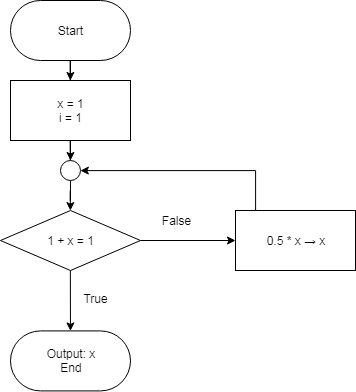
\includegraphics[width=0.4\textwidth]{graphics/machine_epsilon_flowchart}
        \caption{algorithm to find the relative machine precision}\label{fig:epsilon}
      \end{figure}
\end{theorem}

\begin{theorem}
    Using a computer, the relative machine precision can be computed in the following manner
    \begin{equation*}
        \tau = \left|\frac{7}{3} - \frac{3}{4} - 1\right|
    \end{equation*}
\begin{proof}
    We will first evaluate \(\frac{7}{3} - \frac{4}{3}\). We have
    \begin{align}
        \text{rd}_t(\frac{7}{3}) &= \text{rd}_t((10.\overline{01})_2) = \text{rd}_t((0.10\overline{01})_2 \times 2^2) \\
        \text{rd}_t(\frac{4}{3}) &= \text{rd}_t((1.\overline{01})_2) = \text{rd}_t((0.1\overline{01})_2 \times 2^1)
    \end{align}
    The decimal places of the two numbers only differ in placing. Therefore, if we wound the two numbers above one will be rounded up and the other will be rounded down, and we have
    \begin{equation*}
        \left|\text{rd}_t(\frac{7}{3}) - \text{rd}_t(\frac{4}{3})\right| = 2^2 \cdot \sum_{i=1}^{t} \frac{1}{2} - \frac{1}{4} + 0 + \dots + 0 + \frac{1}{2^t} = 1 + \frac{1}{2^t}
    \end{equation*}
    If we subtract \(1\) from the last term, we get \(\tau = \frac{1}{2^t}\) as desired.
\end{proof}
\end{theorem}
For all following examples, let the mantissa length be \(t = 8\) and the exponent of the floating point arithmetic be bounded by \(N_{\text{min}} = -5\) and \(N_{\text{max}} = 8\).
%
% ===================================================================
% (a)
% ===================================================================
%
\begin{exmp} \label{exmp:xmax}
    Given the context as defined above, the largest number that can be represented is \(x_\text{max} = 255\). The calculation is fairly simple; choose the largest exponent possible and fill every digit of the mantissa with ones. In binary, this would be
    \begin{equation*}
        x_\text{max} = (0.11111111)_2 \times 2^8 = (11111111)_2 \text{,}
    \end{equation*}
    or in decimal
    \begin{align*}
        x_\text{max} &= (-1)^{\nu} \cdot 2^N \cdot \sum_{i=1}^{t}x_i \beta^{-i}\\
        &= 2^8 \cdot \left(\frac{1}{2} + \frac{1}{4} + \frac{1}{8} + \frac{1}{16} + \frac{1}{32} + \frac{1}{64} + \frac{1}{128} + \frac{1}{256}\right) \\
        &= 255 \text{.}
    \end{align*}
\end{exmp}
\begin{exmp}
    To find the smallest possible normalized positive value in the defined floating point arithmetic, we proceed similary to the example \ref{exmp:xmax}. Set the exponent as small as possible and fill the mantissa with zero but the first place. We have in binary
    \begin{equation*}
        x_\text{n-min} = (0.10000000)_2 \times 2^{-5} = 0.000001
    \end{equation*}
    which in decimal this translates together
    \begin{equation*}
        x_\text{n-min} = (-1)^{\nu} \cdot 2^N \cdot \sum_{i=1}^{t}x_i \beta^{-i} = 2^{-5} \cdot \frac{1}{2} = \frac{1}{32} = 0.03125
    \end{equation*}
\end{exmp}
\begin{exmp}
    If we do not require the value to be normalized, the smallest possible positive value is much smaller. To find this \(x_\text{min}\), we again set \(N\) to \(-5\) and fill the mantissa with \(0\) except for the last place. We have in binary representation
    \begin{equation*}
        x_\text{min} = (0.00000001)_2 \times 2^{-5} = 0.0000000000001
    \end{equation*}
    and decimal would be
    \begin{equation*}
        x_\text{min} = (-1)^{\nu} \cdot 2^N \cdot \sum_{i=1}^{t}x_i \beta^{-i} = 2^{-5} \times \frac{1}{256} = \frac{1}{8192} = 0.0001220703125
    \end{equation*}
\end{exmp}
\begin{exmp}
    We want to find the margin for the absolute and the relative error. To find the largest possible absolute error, set the exponent to the maximum value and consider two neighboring floating point numbers such as \(1.00000000)_2 \times 2^8\) and \((1.00000001)_2 \times 2^8 = 1\). Worst case scenario, the given number is right in the middle of these two numbers; therefore, the maximum absolute error is \((0.00000001)_2 \times 2^7 = \frac{1}{2}\). This result is also verified by the lemma \ref{XXX}. The same lemma gives us the boundaries for the relative error, \(2^{-8}\). To conclude, we have
    \begin{align*}
        0 &\leq \text{absolute error} \leq \frac{1}{2} \\
        0 &\leq \text{relative error} \leq \frac{2}{256}
    \end{align*}
\end{exmp}

% ===================================================================
% (b)
% ===================================================================

\begin{exmp}
    Let \(z_1 = 67.0\). We want to find the normalized binary form of this integer with ten decimal place accuracy. According to lemma \ref{XXX}, we have
    \begin{align*}
        67.0 \div 2 &= 33.0 + 1 \\
        33.0 \div 2 &= 16.0 + 1 \\
        16.0 \div 2 &= 8.0 + 0 \\
        8.0 \div 2 &= 4.0 + 0 \\
        4.0 \div 2 &= 2.0 + 0 \\
        2.0 \div 2 &= 1.0 + 0 \\
        1.0 \div 2 &= 0.0 + 1 \text{.}
    \end{align*}
    Reading the reminders on the left from bottom to top yields \(z_1 = 67.0 = (1000011)_2\). To normalize this number, we move the decimal point seven digits to the left. Since \(z_1\) only has seven digits, we do not need to cut off any digits. We have
    \begin{equation*}
        z_1 = 67.0 = (0.1000011)_2 \times 2^7
    \end{equation*}
    If one wants to check the validity of the conversion from decimal to binary above, we can check the solution by applying the formula from the other way.
    \begin{equation*}
        (-1)^{\nu} \cdot 2^N \cdot \sum_{i=1}^{t}x_i \beta^{-i} = 2^7 \cdot \left(\frac{1}{2} + \frac{1}{64} + \frac{1}{128}\right) = 128 \cdot \frac{67}{128} = 67
    \end{equation*}
    Now, let's consider the floating point number of \(67.0\). \(N = 7\) is between \(N_{\text{min}} = -5\) and \(N_{\text{max}} = 8\), also \(67.0\) has 7 digits in binary form; therefore, there is no rounding to do which means that \(67.0\) can be represented with the given floating point arithmetic without loss of precision.
    \begin{equation*}
        \text{rd}_8(z_1) = (1.000011)_2 \times 2^6
    \end{equation*}
    Since there is no loss of precision, one can easily conclude that the absolute and relative error of \(67.0\) and \(\text{rd}_8(67.0)\) is zero.
\end{exmp}
\begin{exmp}
    Let \(z_2 = 287.0\). To find the normalized binary form with ten decimal place accuracy, we have
    \begin{align*}
        287.0 \div 2 &= 143.0 + 1 \\
        143.0 \div 2 &= 71.0 + 1 \\
        71.0 \div 2 &= 35.0 + 1 \\
        35.0 \div 2 &= 17.0 + 1 \\
        17.0 \div 2 &= 8.0 + 1 \\
        8.0 \div 2 &= 4.0 + 0 \\
        4.0 \div 2 &= 2.0 + 0 \\
        2.0 \div 2 &= 1.0 + 0 \\
        1.0 \div 2 &= 0.0 + 1 \text{,}
    \end{align*}
    therefore, \(z_2 = 287.0 = (100011111)_2\). Again, there is no need to round any digits. Its normalized binary form is
    \begin{equation*}
        z_2 = 287.0 = (0.100011111)_2 \times 2^9
    \end{equation*}
    In this example, we have an exponent \(N = 9\) which is greater than \(N_{\text{max}} = 8\). This means that with the given floating point arithmetic, we have an overflow and \(287.0\) cannot be rounded to a floating point number. Previously \ref{XXX}, we have shown that \(x_{\text{max}} = 255\) which is another reason why \(z_2 > x_{\text{max}}\) cannot be expressed as a floating point number in this context.
    Most trivially, both absolute and relative error are also undefined for \(287.0\).
\end{exmp}
\begin{exmp}
    For a non-integer example, let \(z_3 = 10.625\). To find the binary form of this number, we first separate \(z_3 = 10.0 + 0.625\) and apply the algorithm of \ref{XXX} on each summand. For \(10.0\) we have
    \begin{align*}
        10.0 \div 2 &= 5.0 + 0 \\
        5.0 \div 2 &= 2.0 + 1 \\
        2.0 \div 2 &= 1.0 + 0 \\
        1.0 \div 2 &= 0.0 + 1
    \end{align*}
    and for \(0.625\) we will multiply it with \(2\) until we get \(0\)
    \begin{align*}
        0.625 \times 2 &= 0.25 + 1 \\
        0.25 \times 2 &= 0.5 + 0 \\
        0.5 \times 2 &= 0.0 + 1
    \end{align*}
    Combining both results together, we get \(z_3 = (1010.101)_2\). To normalize, we move the decimal place three digits to the left and we have
    \begin{equation*}
        z_3 = 10.625 = (1.010101 \times 2^3)_2 \text{.}
    \end{equation*}
\end{exmp}
\begin{exmp}
    Perhaps a more interesting example is needed. Let \(z_4 = 1.01\). As we did in \ref{XXX EXAMPLE ABOVE}, we will separate \(z_4\) in two parts; however, we immediately see that \(1\) is \(1\) in both decimal and binary system. We will therefore consider \(0.01\).
    \begin{align*}
        0.01 \times 2 &= 0.02 + 0 \\
        0.02 \times 2 &= 0.04 + 0 \\
        0.04 \times 2 &= 0.08 + 0 \\
        0.08 \times 2 &= 0.16 + 0 \\
        0.16 \times 2 &= 0.32 + 0 \\
        0.32 \times 2 &= 0.64 + 0 \\
        1.28 \times 2 &= 0.28 + 1 \\
        0.28 \times 2 &= 0.56 + 0 \\
        0.56 \times 2 &= 0.12 + 1 \\
        0.12 \times 2 &= 0.24 + 0
    \end{align*}
    We could go on, but since we only need to find the normalized binary form with respect to ten decimal places. We have
    \begin{equation*}
        z_4 = 1.01 \approx (1.0000001010 \times 2^0)_2
    \end{equation*}
    which is already normalized.
\end{exmp}
\begin{exmp}
    As we already fell into the rabit hole of numbers which have endlessly long binary forms, let's continue with \(z_5 = 0.0002\). For this example, we must stay diligent and iterate many times over the algorithm.
    \begin{align*}
        0.0002 \times 2 &= 0.0004 + 0 \\
        0.0004 \times 2 &= 0.0008 + 0 \\
        0.0008 \times 2 &= 0.0016 + 0 \\
        0.0016 \times 2 &= 0.0032 + 0 \\
        0.0032 \times 2 &= 0.0064 + 0 \\
        0.0064 \times 2 &= 0.0128 + 0 \\
        0.0128 \times 2 &= 0.0256 + 0 \\
        0.0256 \times 2 &= 0.0512 + 0 \\
        0.0512 \times 2 &= 0.1024 + 0 \\
        0.1024 \times 2 &= 0.2048 + 0 \\
        0.2048 \times 2 &= 0.4096 + 0 \\
        0.4096 \times 2 &= 0.8192 + 0 \\
        0.8192 \times 2 &= 0.6384 + 1
    \end{align*}
    We got our first 1! Now we only have to find a maximum of 10 more digits.
    \begin{align*}
        0.6384 \times 2 &= 0.2768 + 1 \\
        0.2768 \times 2 &= 0.5536 + 0 \\
        0.5536 \times 2 &= 0.1072 + 1 \\
        0.1072 \times 2 &= 0.2144 + 0 \\
        0.2144 \times 2 &= 0.4288 + 0 \\
        0.4288 \times 2 &= 0.8576 + 0 \\
        0.8576 \times 2 &= 0.7152 + 1 \\
        0.7152 \times 2 &= 0.4304 + 1 \\
        0.4304 \times 2 &= 0.8608 + 0 \\
        0.8608 \times 2 &= 0.7216 + 1
    \end{align*}
    Therefore, we have \(z_5 = 0.0002 \approx (0.00000000000011010001101)_2\) and normalized we have
    \begin{equation*}
        z_5 = 0.0002 \approx (1.1010001101 \times 2^{-13})_2
    \end{equation*}
\end{exmp}
\begin{exmp}
    For the more mathematically minded, we have last but not least \(z_6 = \frac{1}{3}\).
    \begin{align*}
        \frac{1}{3} \times 2 &= \frac{2}{3} + 0 \\
        \frac{2}{3} \times 2 &= \frac{1}{3} + 1
    \end{align*}
    We already see a patern here; further calculation is not needed. We simply have
    \begin{equation*}
        z_6 = \frac{1}{3} \approx (1.0101010101 \times 2^{-2})_2
    \end{equation*}
\end{exmp}
%
For posterity and stripped from tedious calculation, in the following is a table summerizing the results of \ref{XXX}.
\begin{center}
    \begin{tabular}{| c | c |}
        \hline
        decimal representation & normalized binary representation\\
        \hline
        \(67.0\) & \(1.000011 \times 2^6\) \\
        \(287.0\) & \(1.00011111 \times 2^8\) \\
        \(10.625\) & \(1.010101 \times 2^3\) \\
        \(1.01\) & \(1.0000001010 \times 2^0\) \\
        \(0.0002\) & \(1.1010001101 \times 2^{-13}\) \\
        \(\frac{1}{3}\) & \(1.0101010101 \times 2^{-2}\) \\
        \hline
    \end{tabular}
\end{center}
%
%
% ----------------------------------------------------------------------------------------------------------
% HEADER
% ----------------------------------------------------------------------------------------------------------
%
\documentclass[refman]{scrartcl}
%
\usepackage[english]{babel}
\usepackage{colortbl}
\usepackage{epigraph}
\usepackage{fancyhdr}
\usepackage{graphicx}
\usepackage{hhline}
\usepackage[utf8]{inputenc}
\usepackage[procnames]{listings}
\usepackage{longtable}
\usepackage{tikz}
\usepackage{subcaption}
\usepackage{xcolor}
\usepackage{wrapfig}
\usepackage{amsmath}
%
\usepackage[T1]{fontenc}
\usepackage{lmodern}
%
\pagestyle{fancy}
%
\usetikzlibrary{trees}
%
\definecolor{LightCyan}{rgb}{0.60, 1, 1}
\definecolor{LightGreen}{rgb}{0.56, 0.93, 0.56}
\definecolor{LightGrey}{rgb}{0.83, 0.83, 0.83}
\definecolor{Amber}{rgb}{1.0, 0.75, 0.0}
\definecolor{DarkOrange}{rgb}{1.0, 0.55, 0.0}
\definecolor{DarkGreen}{rgb}{0.15, 0.85, 0.3}
%
\definecolor{deepblue}{rgb}{0,0,0.5}
\definecolor{deepred}{rgb}{0.6,0,0}
\definecolor{deepgreen}{rgb}{0,0.5,0}
%
\definecolor{darkmidnightblue}{rgb}{0.0, 0.2, 0.4}
%
\definecolor{keywords}{rgb}{0.54, 0.17, 0.89}
\definecolor{comments}{RGB}{0,0,113}
\definecolor{raed}{RGB}{160,0,0}
\definecolor{green}{RGB}{0,150,0}
 
\lstset{language=Python,
        numbers=left,
        stepnumber=1,
        breakatwhitespace=true,
        numberstyle=\tiny\color{gray},
        basicstyle=\ttfamily\small, 
        keywordstyle=\color{keywords},
        commentstyle=\fontseries{lc}\selectfont\itshape\color{gray},
        stringstyle=\color{raed},
        showstringspaces=false,
        identifierstyle=\color{darkmidnightblue},
        procnamekeys={def,class}}
%
% ----------------------------------------------------------------------------------------------------------
% TITLEPAGE & TABLE OF CONTENTS
% ----------------------------------------------------------------------------------------------------------
%
\begin{document}
%\begin{titlepage}
	\centering
	
\includegraphics[width=0.15\textwidth]{images/huberlin_logo}\par\vspace{1cm}
	{\scshape\LARGE Humboldt University of Berlin \par}
	\vspace{1cm}
	{\scshape\Large Einf{\"u}hrung in das wissenschaftliche Rechnen \par}
	\vspace{1.5cm}
	{\huge\bfseries Analysis of selected sorting Algorithms\par}
	\vspace{2cm}
	{\Large\itshape Christian Parpart \& Kei Thoma \par}
	\vfill

	\vfill

% Bottom of the page
	{\large \today\par}
\end{titlepage}

\tableofcontents
\newpage
%
% 1 INTRODUCTION
%It is perhaps the most profound realization
%
%\section{Quicksort}
\subsection{Intuition and Description}
Quicksort is a divide-and-conquere, recursive sorting algorithm.\cite[p.~145]{bib:introductiontoalgorithms} Informally speaking, quicksort first chooses a pivot element (in our case, the last element of the list\footnote{For the purpose of this paper, we define a list to be an ordered set for which an order relation such as \(<\) is defined. In terms of computer science, this equates to an array-like data type (in Python this would be a list) with elements which can be compared. An concrete example would be \((0, 1, 2, 3)\) which is incidentally already sorted according to the smaller relation, \(<\).} is chosen as the pivot\footnote{There are more sophisticated ways to choose the pivot. See section XXX for more information.}), then compares every element of the given list to the pivot placing elements smaller than the pivot to the left and every other element to the right. This partitions the list into two. The initial pivot is placed between the two partitions. Note that the pivot is correctly placed since every element smaller than the pivot are in the left partition. Then, the quicksort algorithm is applied to both partitions. The recursion is broken if the current partition only contains zero or one elements.

More formally, we present the pseudocode for the procedure.

\begin{lstlisting}
def partition(_partition, _low, _high):
    i = _low - 1

    # here, we choose the pivot as the far right element of the
    # partition
    pivot = _partition[_high]

    # from line 12 to line 17 we move every element smaller than 
    # the pivot to the left and every other element to the right
    # then we place the pivot in the middle of the two partitions
    for j in range(_low, _high):
        if _partition[j] < pivot:
            ++i
            _partition[i], _partition[j] = _partition[j], 
                                           _partition[i]
    ++i
    _partition[i], _partition[j] = _partition[j], _partition[i]

    return i

def sort_range(_partition, _low, _high):
    if _low < _high:
        pivot_index = partition(_partition)

        if pivot_index > 0:
            sort_range(_partition, _low, pivot_index - 1)
        sort_range(_partition, pivot_index + 1, _high)


# entry point of the algorithm
def quicksort(_list):
    list_length = len(_list)
    sort_range(_list, 0, list_length - 1)

\end{lstlisting}

\subsection{Worked Example}
To demonstrate quicksort concretely, we will apply the algorithm on the list 

\begin{equation*}
    (7, 1, 5, 4, 9, 2, 8, 3, 0, 6) \text{.}
\end{equation*}

\textbf{Color Key}
\begin{itemize}
    \item partitions to be sorted in the following steps are marked with {\color{Amber}orange}
    \item partitions currently ignored are colored in {\color{gray}gray}
    \item pivots are marked with {\color{cyan}teal}
    \item elements which were swapped are in {\color{red}red}
    \item finally, previous pivot element placed correctly after the partitioning are indicated with {\color{green}}
\end{itemize}

\begin{center}
    \begin{longtable}{ | c | c | c | c | c | c | c | c | c | c || l | }
        \hline
        7 & 1 & 5 & 4 & 9 & 2 & 8 & 3 & 0 & 6 &(0) the initial state \\ \hline
        7 & 1 & 5 & 4 & 9 & 2 & 8 & 3 & 0 &\cellcolor{LightCyan}6 &(1) choose \color{cyan}pivot\\ \hline % i = -1
        \color{red}1 & \color{red}7 & 5 & 4 & 9 & 2 & 8 & 3 & 0 &\cellcolor{LightCyan}6 &(2) swap \(\color{red}7\) and \(\color{red}1\)\\ \hline % i = 0
        1 & \color{red}5 & \color{red}7 & 4 & 9 & 2 & 8 & 3 & 0 &\cellcolor{LightCyan}6 &(3) swap \(\color{red}7\) and \(\color{red}5\)\\ \hline % i = 1
        1 & 5 & \color{red}4 & \color{red}7 & 9 & 2 & 8 & 3 & 0 &\cellcolor{LightCyan}6 &(4) swap \(\color{red}7\) and \(\color{red}4\)\\ \hline % i = 2
        1 & 5 & 4 & \color{red}2 & 9 & \color{red} 7 & 8 & 3 & 0 &\cellcolor{LightCyan}6 &(5) swap \(\color{red}7\) and \(\color{red}2\)\\ \hline % i = 3
        1 & 5 & 4 & 2 & \color{red}3 & 7 & 8 & \color{red}9 & 0 &\cellcolor{LightCyan}6 &(6) swap \(\color{red}9\) and \(\color{red}3\)\\ \hline % i = 4
        1 & 5 & 4 & 2 & 3 & \color{red}0 & 8 & 9 & \color{red}7 &\cellcolor{LightCyan}6 &(7) swap \(\color{red}7\) and \(\color{red}0\)\\ \hline % i = 5
        1 & 5 & 4 & 2 & 3 & 0 & \color{cyan}6 & 9 & 7 & \color{red}8 &(8) swap \(\color{red}8\) and the {\color{cyan}pivot}\\ \hline % i = 6 p_i = 6
        1 & 5 & 4 & 2 & 3 & 0 & \cellcolor{LightGreen}6 & 9 & 7 & 8 &(9) \(\color{green}6\) is in the correct place \\ \hhline{===========}
        \multicolumn{11}{ | c | }{partition the sequence into \((1, 5, 4, 2, 3, 0)\) and \((9, 7, 8)\)} \\ \hhline{===========}
        \cellcolor{Amber}1 & \cellcolor{Amber}5 & \cellcolor{Amber}4 & \cellcolor{Amber}2 & \cellcolor{Amber}3 & \cellcolor{Amber}0 & \cellcolor{LightGreen}6 & \cellcolor{LightGrey}9 & \cellcolor{LightGrey}7 & \cellcolor{LightGrey}8 &(10) sort {\color{DarkOrange}left side} \\ \hline
        1 & 5 & 4 & 2 & 3 & \cellcolor{LightCyan}0 & \cellcolor{LightGreen}6 & \cellcolor{LightGrey}9 & \cellcolor{LightGrey}7 & \cellcolor{LightGrey}8 &(11) choose {\color{cyan}pivot} \\ \hline
        \color{cyan}0 & 5 & 4 & 2 & 3 & \color{red}1 & \cellcolor{LightGreen}6 & \cellcolor{LightGrey}9 & \cellcolor{LightGrey}7 & \cellcolor{LightGrey}8 &(12) swap \(\color{red}1\) and the {\color{cyan}pivot}\\ \hline
        \cellcolor{LightGreen}0 & 5 & 4 & 2 & 3 & 1 & \cellcolor{LightGreen}6 & \cellcolor{LightGrey}9 & \cellcolor{LightGrey}7 & \cellcolor{LightGrey}8 &(13) {\color{green}0} is in the correct place\\ \hhline{===========}
        \multicolumn{11}{ | c | }{partition the sequence into \(()\) and \((5, 4, 2, 3, 1)\)} \\ \hhline{===========}
        \cellcolor{LightGreen}0 & \cellcolor{LightGrey}5 & \cellcolor{LightGrey}4 & \cellcolor{LightGrey}2 & \cellcolor{LightGrey}3 & \cellcolor{LightGrey}1 & \cellcolor{LightGreen}6 & \cellcolor{LightGrey}9 & \cellcolor{LightGrey}7 & \cellcolor{LightGrey}8 &(14) nothing to sort on the {\color{DarkOrange}left side}\\ \hline
        \cellcolor{LightGreen}0 & \cellcolor{Amber}5 & \cellcolor{Amber}4 & \cellcolor{Amber}2 & \cellcolor{Amber}3 & \cellcolor{Amber}1 & \cellcolor{LightGreen}6 & \cellcolor{LightGrey}9 & \cellcolor{LightGrey}7 & \cellcolor{LightGrey}8 &(15) sort {\color{DarkOrange}right side}\\ \hline
        \cellcolor{LightGreen}0 & 5 & 4 & 2 & 3 & \cellcolor{LightCyan}1 & \cellcolor{LightGreen}6 & \cellcolor{LightGrey}9 & \cellcolor{LightGrey}7 & \cellcolor{LightGrey}8 &(16) choose {\color{cyan}pivot} \\ \hline
        \cellcolor{LightGreen}0 & \color{cyan}1 & 4 & 2 & 3 & \color{red}5 & \cellcolor{LightGreen}6 & \cellcolor{LightGrey}9 & \cellcolor{LightGrey}7 & \cellcolor{LightGrey}8 &(17) swap \(\color{red}5\) and the {\color{cyan}pivot} \\ \hline
        \cellcolor{LightGreen}0 & \cellcolor{LightGreen}1 & 4 & 2 & 3 & 5 & \cellcolor{LightGreen}6 & \cellcolor{LightGrey}9 & \cellcolor{LightGrey}7 & \cellcolor{LightGrey}8 &(18) {\color{green}1} is in the correct place \\ \hhline{===========}
        \multicolumn{11}{ | c | }{partition the sequence into \(()\) and \((4, 2, 3, 5)\)} \\ \hhline{===========}
        \cellcolor{LightGreen}0 & \cellcolor{LightGreen}1 & \cellcolor{LightGrey}4 & \cellcolor{LightGrey}2 & \cellcolor{LightGrey}3 & \cellcolor{LightGrey}5 & \cellcolor{LightGreen}6 & \cellcolor{LightGrey}9 & \cellcolor{LightGrey}7 & \cellcolor{LightGrey}8 &(19) nothing to sort on the {\color{DarkOrange}left side}\\ \hline
        \cellcolor{LightGreen}0 & \cellcolor{LightGreen}1 & \cellcolor{Amber}4 & \cellcolor{Amber}2 & \cellcolor{Amber}3 & \cellcolor{Amber}5 & \cellcolor{LightGreen}6 & \cellcolor{LightGrey}9 & \cellcolor{LightGrey}7 & \cellcolor{LightGrey}8 &(20) sort {\color{DarkOrange}right side}\\ \hline
        \cellcolor{LightGreen}0 & \cellcolor{LightGreen}1 & 4 & 2 & 3 & \cellcolor{LightCyan}5 & \cellcolor{LightGreen}6 & \cellcolor{LightGrey}9 & \cellcolor{LightGrey}7 & \cellcolor{LightGrey}8 &(21) choose {\color{cyan}pivot} \\ \hline
        \cellcolor{LightGreen}0 & \cellcolor{LightGreen}1 & 4 & 2 & 3 & \cellcolor{LightGreen}5 & \cellcolor{LightGreen}6 & \cellcolor{LightGrey}9 & \cellcolor{LightGrey}7 & \cellcolor{LightGrey}8 &(22) \(\color{green}5\) is in the correct place \\ \hhline{===========}
        \multicolumn{11}{ | c | }{partition the sequence into \((4, 2, 3)\) and \(()\)} \\ \hhline{===========}
        \cellcolor{LightGreen}0 & \cellcolor{LightGreen}1 & \cellcolor{Amber}4 & \cellcolor{Amber}2 & \cellcolor{Amber}3 & \cellcolor{LightGreen}5 & \cellcolor{LightGreen}6 & \cellcolor{LightGrey}9 & \cellcolor{LightGrey}7 & \cellcolor{LightGrey}8 &(23) sort {\color{DarkOrange}left side} \\ \hline
        \cellcolor{LightGreen}0 & \cellcolor{LightGreen}1 & 4 & 2 & \cellcolor{LightCyan}3 & \cellcolor{LightGreen}5 & \cellcolor{LightGreen}6 & \cellcolor{LightGrey}9 & \cellcolor{LightGrey}7 & \cellcolor{LightGrey}8 &(24) choose {\color{cyan}pivot} \\ \hline
        \cellcolor{LightGreen}0 & \cellcolor{LightGreen}1 & \color{red}2 & \color{red}4 & \cellcolor{LightCyan}3 & \cellcolor{LightGreen}5 & \cellcolor{LightGreen}6 & \cellcolor{LightGrey}9 & \cellcolor{LightGrey}7 & \cellcolor{LightGrey}8 &(25) swap \(\color{red}4\) and \(\color{red}2\) \\ \hline
        \cellcolor{LightGreen}0 & \cellcolor{LightGreen}1 & 2 & \color{cyan}3 & \color{red}4 & \cellcolor{LightGreen}5 & \cellcolor{LightGreen}6 & \cellcolor{LightGrey}9 & \cellcolor{LightGrey}7 & \cellcolor{LightGrey}8 &(26) swap \(\color{red}4\) and the {\color{cyan}pivot} \\ \hline
        \cellcolor{LightGreen}0 & \cellcolor{LightGreen}1 & 2 & \cellcolor{LightGreen}3 & 4 & \cellcolor{LightGreen}5 & \cellcolor{LightGreen}6 & \cellcolor{LightGrey}9 & \cellcolor{LightGrey}7 & \cellcolor{LightGrey}8 &(27) \(\color{LightGreen}3\) is in the correct place \\ \hline
        \cellcolor{LightGreen}0 & \cellcolor{LightGreen}1 & \cellcolor{LightGrey}2 & \cellcolor{LightGreen}3 & \cellcolor{LightGrey}4 & \cellcolor{LightGreen}5 & \cellcolor{LightGreen}6 & \cellcolor{LightGrey}9 & \cellcolor{LightGrey}7 & \cellcolor{LightGrey}8 &(28) nothing to sort on the {\color{DarkOrange}right side} \\ \hhline{===========}
        \multicolumn{11}{ | c | }{partition the sequence into \((2)\) and \((4)\)} \\ \hhline{===========}
        \cellcolor{LightGreen}0 & \cellcolor{LightGreen}1 & \cellcolor{Amber}2 & \cellcolor{LightGreen}3 & \cellcolor{LightGrey}4 & \cellcolor{LightGreen}5 & \cellcolor{LightGreen}6 & \cellcolor{LightGrey}9 & \cellcolor{LightGrey}7 & \cellcolor{LightGrey}8 &(27) sort {\color{DarkOrange}left side} \\ \hline
        \cellcolor{LightGreen}0 & \cellcolor{LightGreen}1 & \cellcolor{LightGreen}2 & \cellcolor{LightGreen}3 & \cellcolor{LightGrey}4 & \cellcolor{LightGreen}5 & \cellcolor{LightGreen}6 & \cellcolor{LightGrey}9 & \cellcolor{LightGrey}7 & \cellcolor{LightGrey}8 &(28) \(\color{green}2\) is in the correct place \\ \hline
        \cellcolor{LightGreen}0 & \cellcolor{LightGreen}1 & \cellcolor{LightGreen}2 & \cellcolor{LightGreen}3 & \cellcolor{Amber}4 & \cellcolor{LightGreen}5 & \cellcolor{LightGreen}6 & \cellcolor{LightGrey}9 & \cellcolor{LightGrey}7 & \cellcolor{LightGrey}8 &(29) sort {\color{DarkOrange}right side} \\ \hline
        \cellcolor{LightGreen}0 & \cellcolor{LightGreen}1 & \cellcolor{LightGreen}2 & \cellcolor{LightGreen}3 & \cellcolor{LightGreen}4 & \cellcolor{LightGreen}5 & \cellcolor{LightGreen}6 & \cellcolor{LightGrey}9 & \cellcolor{LightGrey}7 & \cellcolor{LightGrey}8 &(30) \(\color{green}4\) is in the correct place \\ \hhline{===========} \hhline{===========}
        \cellcolor{LightGreen}0 & \cellcolor{LightGreen}1 & \cellcolor{LightGreen}2 & \cellcolor{LightGreen}3 & \cellcolor{LightGreen}4 & \cellcolor{LightGreen}5 & \cellcolor{LightGreen}6 & \cellcolor{Amber}9 & \cellcolor{Amber}7 & \cellcolor{Amber}8 &(31) sort {\color{DarkOrange}right side} \\ \hline
        \cellcolor{LightGreen}0 & \cellcolor{LightGreen}1 & \cellcolor{LightGreen}2 & \cellcolor{LightGreen}3 & \cellcolor{LightGreen}4 & \cellcolor{LightGreen}5 & \cellcolor{LightGreen}6 & 9 & 7 & \cellcolor{LightCyan}8 &(32) choose {\color{cyan}pivot} \\ \hline
        \cellcolor{LightGreen}0 & \cellcolor{LightGreen}1 & \cellcolor{LightGreen}2 & \cellcolor{LightGreen}3 & \cellcolor{LightGreen}4 & \cellcolor{LightGreen}5 & \cellcolor{LightGreen}6 & \color{red}7 & \color{red}9 & \cellcolor{LightCyan}8 &(33) swap \(\color{red}9\) and \(\color{red}7\) \\ \hline
        \cellcolor{LightGreen}0 & \cellcolor{LightGreen}1 & \cellcolor{LightGreen}2 & \cellcolor{LightGreen}3 & \cellcolor{LightGreen}4 & \cellcolor{LightGreen}5 & \cellcolor{LightGreen}6 & 7 & \color{cyan}8 & \color{red}9 &(34) swap \(\color{red}9\) and {\color{cyan}pivot} \\ \hline
        \cellcolor{LightGreen}0 & \cellcolor{LightGreen}1 & \cellcolor{LightGreen}2 & \cellcolor{LightGreen}3 & \cellcolor{LightGreen}4 & \cellcolor{LightGreen}5 & \cellcolor{LightGreen}6 & 7 & \cellcolor{LightGreen}8 & 9 &(35) \(\color{green}8\) is in the correct place \\ \hhline{===========}
        \multicolumn{11}{ | c | }{partition the sequence into \((7)\) and \((9)\)} \\ \hhline{===========}
        \cellcolor{LightGreen}0 & \cellcolor{LightGreen}1 & \cellcolor{LightGreen}2 & \cellcolor{LightGreen}3 & \cellcolor{LightGreen}4 & \cellcolor{LightGreen}5 & \cellcolor{LightGreen}6 & \cellcolor{Amber}7 & \cellcolor{LightGreen}8 & \cellcolor{LightGrey}9 &(36) sort {\color{DarkOrange}left side} \\ \hline
        \cellcolor{LightGreen}0 & \cellcolor{LightGreen}1 & \cellcolor{LightGreen}2 & \cellcolor{LightGreen}3 & \cellcolor{LightGreen}4 & \cellcolor{LightGreen}5 & \cellcolor{LightGreen}6 & \cellcolor{LightGreen}7 & \cellcolor{LightGreen}8 & \cellcolor{LightGrey}9 &(37) \(\color{green}7\) is in the correct place \\ \hline
        \cellcolor{LightGreen}0 & \cellcolor{LightGreen}1 & \cellcolor{LightGreen}2 & \cellcolor{LightGreen}3 & \cellcolor{LightGreen}4 & \cellcolor{LightGreen}5 & \cellcolor{LightGreen}6 & \cellcolor{LightGreen}7 & \cellcolor{LightGreen}8 & \cellcolor{Amber}9 &(38) sort {\color{DarkOrange}left side} \\ \hline
        \cellcolor{LightGreen}0 & \cellcolor{LightGreen}1 & \cellcolor{LightGreen}2 & \cellcolor{LightGreen}3 & \cellcolor{LightGreen}4 & \cellcolor{LightGreen}5 & \cellcolor{LightGreen}6 & \cellcolor{LightGreen}7 & \cellcolor{LightGreen}8 & \cellcolor{LightGreen}9 &(39) \(\color{green}9\) is in the correct place \\ \hline
        \cellcolor{LightGreen}0 & \cellcolor{LightGreen}1 & \cellcolor{LightGreen}2 & \cellcolor{LightGreen}3 & \cellcolor{LightGreen}4 & \cellcolor{LightGreen}5 & \cellcolor{LightGreen}6 & \cellcolor{LightGreen}7 & \cellcolor{LightGreen}8 & \cellcolor{LightGreen}9 &(40) every thing is correctly sorted \\ \hline
        \caption{An example of quicksort applied to the sequence \((7, 1, 5, 4, 9, 2, 8, 3, 0, 6)\). Note that the table above is presented purely to illustrate the procedure of the algorithm and may not reflect one-to-one its implementation on a computer. For example, before swapping two numbers, the algorithm needs to compare each number leading up to that number to the pivot which was skipped in the table to improve readability. The numbers in the parentheses in the most right columns are also merely for referencing a specific row and do not correlate with the number of steps the algorithm needs to sort the given sequence.} \\
    \end{longtable}
\end{center}

We start with a sequence \((7, 1, 5, 4, 9, 2, 8, 3, 0, 6)\) which has ten distinct elements from \(0\) to \(9\). The far right element, \(6\), is chosen as the pivot (row 1). At the same time, define a counter \(i\) and set it to \(-1\). Then, start comparing each element from the left to right to the pivot. If the element is larger (or equal) than the pivot, nothing happens, but if it is smaller than the pivot, increment \(i\) by one and swap the number that was compared to the pivot with the number on \(i\)-th place of the sequence. For example, \(7 > 6\) hence nothing is changed, but \(1 < 6\) therefore, \(i\) is set to \(0\) and \(5\) is swapped with the number on the \(0\)th place which is \(7\) (row 2). The next number \(5\) is also smaller than the pivot \(6\), therefore, \(i\) is increment to \(1\) and \(5\) is swapped with the number on the first place which is again \(7\). This procedure is done for each number (compare rows 3 to 7). Finally, the pivot is swapped with the number on the \(i\)-th place. In our case, \(i\) is \(6\) at the end and the initial pivot \(6\) is correctly placed after the swap (see rows 8 and 9).

After placing the initial pivot correctly, the sequence is partitioned into the left and the right side of the pivot which only contain numbers smaller or larger (or equal) than the pivot respectively i.e. the two partitions are \((1, 5, 4, 2, 3, 0)\) and \((9, 7, 8)\) with the first partition containing only numbers smaller than the pivot. Now, quicksort which is a recursive algorithm is applied to both partitions. For example, in the left partition, \(0\) is chosen as the pivot (row 11).

There are few interesting points. On row 14, the first partition is empty, therefore nothing is sorted. Few rows after in row 22, we bluntly wrote that \(5\) is in the correct place, but we've skipped multiple steps before. In actuallity, because every number in the partition \((4, 2, 3, 5)\) are smaller (or equal) to the pivot \(5\) they are all swapped with themselves i.e. \(4\) is swapped with \(4\) and \(2\) is swapped with \(2\) and so on.

\subsection{Complexity}
%The complexity of quicksort highly depends on the choice of the pivot. We set the pivot naïvely to be the last element in the partition which is not optimal. The best selection of the pivot is the median of the list since this would leave half of the elements on the left and the other half on the right of the pivot splitting the list into two equally large partitions.

%Therefore, we call a pivot \textit{good enough} if it lies in the center half of the list i.e. larger than the smallest 1/4, but smaller than the largest 3/4. In the worst case scenario for a good enough pivot, the larger partition has the 3/4 of the size of the intial list. Following the recursion, we get partitions in sizes of
%\begin{equation*}
%    n, \frac{3}{4} n, \left(\frac{3}{4}\right)^2 n, \dots, 1 \text{.}
%\end{equation*}
%Let \(h_g\) be the height of the quicksort partition tree. Then for \(\left(\frac{3}{4}\right)^{h_g} n = 1\) we have \(\)

The complexity of quicksort highly depends on the choice of the pivot. We have set the pivot naïvely to be the last element in the partition which is not optimal. In general, a median pivot is the most desireble since it splits the list into two most possible even partitions.

The worst case for quicksort is when every recursion creates a partition of maximum length. This results in the complexity of \(O(n^2)\) (same as selection sort). While a very rare case, this happens most interestingly when the list is already sorted due to the nature how we pick our pivot.\cite[p.~137]{bib:thealgorithmdesignmanual}

If every split produces partition with equal length (or length differing exactly by one), the algorithm achives the best case performance of \(O(n \ln(n))\). The average case of quicksort is closer to the best case than to the worst case. Indeed, the average case running time of quicksort is again \(O(n \ln(n))\).\cite[p.~150]{bib:introductiontoalgorithms}

Quicksort is not stable. We will show this with an example. Consider a list \((2, 2^{*}, 1)\). After choosing \(1\) as the initial pivot, the list is sorted almost immediately into \((1, 2^{*}, 2)\). \(2\) and \(2^{*}\) do not retain their order, hence quicksort is not stable.
%
\section{Heapsort}
\subsection{Intuition and Description}
Heapsort is a sorting algorithm which introduces a data structure, a binary tree (the \textit{heap}). A heap is a nearly complete binary tree. For example, consider the list from previous examples

\begin{equation*}
    (7, 1, 5, 4, 9, 2, 8, 3, 0, 6) \text{.}
\end{equation*}

This list can be arranged into a heap simply by placing the first element of the list at the root, then placing the next two elements as its children and so on (see figure \ref{fig:heap}).
\begin{wrapfigure}{r}{0.5\textwidth}
    \begin{tikzpicture}[level distance=1cm,
        level 1/.style={sibling distance=3cm},
        level 2/.style={sibling distance=1.5cm},
        level 3/.style={sibling distance=1cm}]
        \node {7}
            child {
                node {1}
                child {
                    node {4}
                    child {
                        node {3}
                    }
                    child {
                        node {0}
                    }
                }
                child {
                    node {9}
                    child {
                        node {6}
                    }
                }
            }
            child {
                node {5}
                child {
                    node {2}
                }
                child {
                    node {8}
                }
            };
    \end{tikzpicture}
    \caption{the given list arranged into a heap}\label{fig:heap}
\end{wrapfigure}

In essence, the goal of heapsort is to first sort the heap into a \textit{max-heap} where each parent is larger than each of its children. Then, the root element which by necessity must be the largest element is removed from the heap and the element on the lowest branch (in figure \ref{fig:heap} where 6 currently is) is moved to the root (this procedure as a function is called \textit{build-max-heap}).

It turns out however, that not every recursion needs to check if the heap is a max-heap. After sorting the initial heap, one can assume that the heap is already sorted except for the root. The function which partially sorts the heap after the largest element was removed and the element of the lowest branch is moved to the top is called \textit{heapify}.\cite[p.~135]{bib:introductiontoalgorithms} 

As we did with quicksort, we present the pseudocode for heapsort in the following.

\begin{lstlisting}
def heapsort(_list):
    def heapify(_list, _n, _i):
        largest_element_index = _i

        LEFT_CHILD_INDEX = 2 * _i + 1
        if LEFT_CHILD_INDEX < _n:
            if (_list[LEFT_CHILD_INDEX] > 
                _list[largest_element_index]):
                largest_element_index = LEFT_CHILD_INDEX
    
        RIGHT_CHILD_INDEX = 2 * _i + 2
        IF RIGHT_CHILD_INDEX < _n:
            if (_list[RIGHT_CHILD_INDEX] >
                _list[largest_element_index]):
                largest_element_index = RIGHT_CHILD_INDEX
        
        if largest_element_index != _i:
            _list[_i], _list[largest_element_index] =
              _list[largest_element_index], _list[_i]

            heapify(_list, _n, largest_element_index)
            
    i = floor(len(_list) / 2) - 1

    while i >= 0:
        heapify(_list, len(_list), i)
        --i
    
    i = len(_list) - 1
    while i >= 0:
        _list[0], _list[i] = _list[0], _list[i]
        heapify(_list, i, 0)
        --i
\end{lstlisting}

\subsection{Worked Example}
As before, consider the list

\begin{equation*}
    (7, 1, 5, 6, 9, 2, 8, 3, 0, 6)\text{.}
\end{equation*}

We will sort this list using heapsort in the following (see figure \ref{fig:heapsortexample}). Due to space restrictions, steps between max heaps were condensed into one.

\textbf{Color Key}

\begin{itemize}
    \item the numbers swapped in the last step are in {\color{red}red} and {\color{green}green}, where {\color{green}green} indicates that the number was previously the root of the heap
    \item numbers {\color{gray}grayed} out are the numbers which are correctly sorted (removed from the heap)
\end{itemize}
\subsection{Complexity}

The initial build-max-heap takes time \(O(n)\) and heapify which takes time \(O(\ln(n))\) and is called \(n - 1\) times. Together, this means that the complexity of heapsort is \(O(n \ln(n))\).\cite[p.~136]{bib:introductiontoalgorithms}

Heapsort is not stable. Consider the following list \(2^{*}, 1, 2
)\). If heapsort is applied, this list is sorted to \(2, 1, 2^{*}\) thus the algorithm is unstable.

\begin{center}
%
% 1 to 10
%
\begin{figure}
    \caption{Worked example of heapsort.}\label{fig:heapsortexample}
    \begin{subfigure}[c]{0.5\textwidth}
    \begin{tikzpicture}[level distance=1cm,
        level 1/.style={sibling distance=3cm},
        level 2/.style={sibling distance=1.5cm},
        level 3/.style={sibling distance=1cm}]
        \node {7}
            child {
                node {1}
                child {
                    node {4}
                    child {
                        node {3}
                    }
                    child {
                        node {0}
                    }
                }
                child {
                    node {9}
                    child {
                        node {6}
                    }
                }
            }
            child {
                node {5}
                child {
                    node {2}
                }
                child {
                    node {8}
                }
            };
    \end{tikzpicture}
    \begin{tabular}{ | c | c | c | c | c | c | c | c | c | c | }
        \hline
        7 & 1 & 5 & 4 & 9 & 2 & 8 & 3 & 0 & 6 \\ \hline
    \end{tabular}
    \caption{(0) initial state}
    \end{subfigure}
    \begin{subfigure}[c]{0.5\textwidth}
    \begin{tikzpicture}[level distance=1cm,
        level 1/.style={sibling distance=3cm},
        level 2/.style={sibling distance=1.5cm},
        level 3/.style={sibling distance=1cm}]
        \node {\color{red}1}
            child {
                node {7}
                child {
                    node {4}
                    child {
                        node {3}
                    }
                    child {
                        node {0}
                    }
                }
                child {
                    node {6}
                    child {
                        node {\color{DarkGreen}9}
                    }
                }
            }
            child {
                node {8}
                child {
                    node {2}
                }
                child {
                    node {5}
                }
            };
    \end{tikzpicture}
    \begin{tabular}{ | c | c | c | c | c | c | c | c | c | c | }
        \hline
        \color{red}1 & 7 & 8 & 4 & 6 & 2 & 5 & 3 & 0 & \color{DarkGreen}9 \\ \hline
    \end{tabular}
    \caption{(1) create max heap; then swap {\color{red}1} and {\color{DarkGreen}9}}
    \end{subfigure}
    \begin{subfigure}[c]{0.5\textwidth}
    \begin{tikzpicture}[level distance=1cm,
        level 1/.style={sibling distance=3cm},
        level 2/.style={sibling distance=1.5cm},
        level 3/.style={sibling distance=1cm}]
        \node {\color{red}0}
            child {
                node {7}
                child {
                    node {4}
                    child {
                        node {3}
                    }
                    child {
                        node {\color{DarkGreen}8}
                    }
                }
                child {
                    node {6}
                    child {
                        [LightGrey]
                        node {\color{LightGrey}9}
                    }
                }
            }
            child {
                node {5}
                child {
                    node {2}
                }
                child {
                    node {1}
                }
            };
    \end{tikzpicture}
    \begin{tabular}{ | c | c | c | c | c | c | c | c | c | c | }
        \hline
        \color{red}0 & 7 & 5 & 4 & 6 & 2 & 1 & 3 & \color{DarkGreen}8 & \color{gray}9 \\ \hline
    \end{tabular}
    \caption{(2) create max heap; swap {\color{red}0} and {\color{DarkGreen}8}}
    \end{subfigure}
    \begin{subfigure}[c]{0.5\textwidth}
    \begin{tikzpicture}[level distance=1cm,
        level 1/.style={sibling distance=3cm},
        level 2/.style={sibling distance=1.5cm},
        level 3/.style={sibling distance=1cm}]
        \node {\color{red}3}
            child {
                node {6}
                child {
                    node {4}
                    child {
                        node {\color{DarkGreen}7}
                    }
                    child {
                        [LightGrey]
                        node {\color{LightGrey}8}
                    }
                }
                child {
                    node {0}
                    child {
                        [LightGrey]
                        node {\color{LightGrey}9}
                    }
                }
            }
            child {
                node {5}
                child {
                    node {2}
                }
                child {
                    node {1}
                }
            };
    \end{tikzpicture}
    \begin{tabular}{ | c | c | c | c | c | c | c | c | c | c | }
        \hline
        \color{red}3 & 6 & 5 & 4 & 0 & 2 & 1 & \color{DarkGreen}7 & \color{gray}8 & \color{gray}9 \\ \hline
    \end{tabular}
    \caption{(3) create max heap; swap {\color{red}3} and {\color{DarkGreen}7}}
    \end{subfigure}
    \begin{subfigure}[c]{0.5\textwidth}
    \begin{tikzpicture}[level distance=1cm,
        level 1/.style={sibling distance=3cm},
        level 2/.style={sibling distance=1.5cm},
        level 3/.style={sibling distance=1cm}]
        \node {\color{red}1}
            child {
                node {4}
                child {
                    node {3}
                    child {
                        [LightGrey]
                        node {\color{LightGrey}7}
                    }
                    child {
                        [LightGrey]
                        node {\color{LightGrey}8}
                    }
                }
                child {
                    node {0}
                    child {
                        [LightGrey]
                        node {\color{LightGrey}9}
                    }
                }
            }
            child {
                node {5}
                child {
                    node {2}
                }
                child {
                    node {\color{DarkGreen}6}
                }
            };
    \end{tikzpicture}
    \begin{tabular}{ | c | c | c | c | c | c | c | c | c | c | }
        \hline
        \color{red}1 & 4 & 5 & 3 & 0 & 2 & \color{DarkGreen}6 & \color{gray}7 & \color{gray}8 & \color{gray}9 \\ \hline
    \end{tabular}
    \caption{(4) create max heap; swap {\color{red}1} and {\color{DarkGreen}6}}
    \end{subfigure}
    \begin{subfigure}[c]{0.5\textwidth}
    \begin{tikzpicture}[level distance=1cm,
        level 1/.style={sibling distance=3cm},
        level 2/.style={sibling distance=1.5cm},
        level 3/.style={sibling distance=1cm}]
        \node {\color{red}1}
            child {
                node {4}
                child {
                    node {3}
                    child {
                        [LightGrey]
                        node {\color{LightGrey}7}
                    }
                    child {
                        [LightGrey]
                        node {\color{LightGrey}8}
                    }
                }
                child {
                    node {0}
                    child {
                        [LightGrey]
                        node {\color{LightGrey}9}
                    }
                }
            }
            child {
                node {2}
                child {
                    node {\color{DarkGreen}5}
                }
                child {
                    [LightGrey]
                    node {\color{LightGrey}6}
                }
            };
    \end{tikzpicture}
    \begin{tabular}{ | c | c | c | c | c | c | c | c | c | c | }
        \hline
        \color{red}1 & 4 & 2 & 3 & 0 & \color{DarkGreen}5 & \color{gray}6 & \color{gray}7 & \color{gray}8 & \color{gray}9 \\ \hline
    \end{tabular}
    \caption{(5) create max heap; swap {\color{red}1} and {\color{DarkGreen}5}}
    \end{subfigure}
        \begin{subfigure}[c]{0.5\textwidth}
        \begin{tikzpicture}[level distance=1cm,
            level 1/.style={sibling distance=3cm},
            level 2/.style={sibling distance=1.5cm},
            level 3/.style={sibling distance=1cm}]
            \node {\color{red}0}
                child {
                    node {3}
                    child {
                        node {1}
                        child {
                            [LightGrey]
                            node {\color{LightGrey}7}
                        }
                        child {
                            [LightGrey]
                            node {\color{LightGrey}8}
                        }
                    }
                    child {
                        node {\color{DarkGreen}4}
                        child {
                            [LightGrey]
                            node {\color{LightGrey}9}
                        }
                    }
                }
                child {
                    node {2}
                    child {
                        [LightGrey]
                        node {\color{LightGrey}5}
                    }
                    child {
                        [LightGrey]
                        node {\color{LightGrey}6}
                    }
                };
    \end{tikzpicture}
    \begin{tabular}{ | c | c | c | c | c | c | c | c | c | c | }
        \hline
        \color{red}0 & 3 & 2 & 1 & \color{DarkGreen}4 & \color{gray}5 & \color{gray}6 & \color{gray}7 & \color{gray}8 & \color{gray}9 \\ \hline
    \end{tabular}
    \caption{(6) create max heap; swap {\color{red}0} and {\color{DarkGreen}4}}
    \end{subfigure}
    \begin{subfigure}[c]{0.5\textwidth}
        \begin{tikzpicture}[level distance=1cm,
            level 1/.style={sibling distance=3cm},
            level 2/.style={sibling distance=1.5cm},
            level 3/.style={sibling distance=1cm}]
            \node {\color{red}0}
                child {
                    node {1}
                    child {
                        node {\color{DarkGreen}3}
                        child {
                            [LightGrey]
                            node {\color{LightGrey}7}
                        }
                        child {
                            [LightGrey]
                            node {\color{LightGrey}8}
                        }
                    }
                    child {
                        [LightGrey]
                        node {\color{LightGrey}4}
                        child {
                            [LightGrey]
                            node {\color{LightGrey}9}
                        }
                    }
                }
                child {
                    node {2}
                    child {
                        [LightGrey]
                        node {\color{LightGrey}5}
                    }
                    child {
                        [LightGrey]
                        node {\color{LightGrey}6}
                    }
                };
    \end{tikzpicture}
    \begin{tabular}{ | c | c | c | c | c | c | c | c | c | c | }
        \hline
        \color{red}0 & 1 & 2 & \color{DarkGreen}3 & \color{gray}4 & \color{gray}5 & \color{gray}6 & \color{gray}7 & \color{gray}8 & \color{gray}9 \\ \hline
    \end{tabular}
    \caption{(7) create max heap; swap {\color{red}0} and {\color{DarkGreen}3}}
    \end{subfigure}
\end{figure}
\begin{figure}
    \begin{subfigure}[c]{0.5\textwidth}
        \begin{tikzpicture}[level distance=1cm,
            level 1/.style={sibling distance=3cm},
            level 2/.style={sibling distance=1.5cm},
            level 3/.style={sibling distance=1cm}]
            \node {\color{red}0}
                child {
                    node {1}
                    child {
                        [LightGrey]
                        node {\color{LightGrey}3}
                        child {
                            [LightGrey]
                            node {\color{LightGrey}7}
                        }
                        child {
                            [LightGrey]
                            node {\color{LightGrey}8}
                        }
                    }
                    child {
                        [LightGrey]
                        node {\color{LightGrey}4}
                        child {
                            [LightGrey]
                            node {\color{LightGrey}9}
                        }
                    }
                }
                child {
                    node {\color{DarkGreen}2}
                    child {
                        [LightGrey]
                        node {\color{LightGrey}5}
                    }
                    child {
                        [LightGrey]
                        node {\color{LightGrey}6}
                    }
                };
    \end{tikzpicture}
    \begin{tabular}{ | c | c | c | c | c | c | c | c | c | c | }
        \hline
        \color{red}0 & 1 & \color{DarkGreen}2 & \color{gray}3 & \color{gray}4 & \color{gray}5 & \color{gray}6 & \color{gray}7 & \color{gray}8 & \color{gray}9 \\ \hline
    \end{tabular}
    \caption{(8) create max heap; swap {\color{red}0} and {\color{DarkGreen}2}}
    \end{subfigure}
    \begin{subfigure}[c]{0.5\textwidth}
        \begin{tikzpicture}[level distance=1cm,
            level 1/.style={sibling distance=3cm},
            level 2/.style={sibling distance=1.5cm},
            level 3/.style={sibling distance=1cm}]
            \node {\color{red}0}
                child {
                    node {\color{DarkGreen}1}
                    child {
                        [LightGrey]
                        node {\color{LightGrey}3}
                        child {
                            [LightGrey]
                            node {\color{LightGrey}7}
                        }
                        child {
                            [LightGrey]
                            node {\color{LightGrey}8}
                        }
                    }
                    child {
                        [LightGrey]
                        node {\color{LightGrey}4}
                        child {
                            [LightGrey]
                            node {\color{LightGrey}9}
                        }
                    }
                }
                child {
                    [LightGrey]
                    node {\color{LightGrey}2}
                    child {
                        [LightGrey]
                        node {\color{LightGrey}5}
                    }
                    child {
                        [LightGrey]
                        node {\color{LightGrey}6}
                    }
                };
    \end{tikzpicture}
    \begin{tabular}{ | c | c | c | c | c | c | c | c | c | c | }
        \hline
        \color{red}0 & \color{DarkGreen}1 & \color{gray}2 & \color{gray}3 & \color{gray}4 & \color{gray}5 & \color{gray}6 & \color{gray}7 & \color{gray}8 & \color{gray}9 \\ \hline
    \end{tabular}
    \caption{(9) create max heap; swap {\color{red}0} and {\color{DarkGreen}1}}
    \end{subfigure}
    \begin{subfigure}[c]{0.5\textwidth}
        \begin{tikzpicture}[level distance=1cm,
            level 1/.style={sibling distance=3cm},
            level 2/.style={sibling distance=1.5cm},
            level 3/.style={sibling distance=1cm}]
            \node {\color{DarkGreen}0}
                child {
                    [LightGrey]
                    node {\color{LightGrey}1}
                    child {
                        [LightGrey]
                        node {\color{LightGrey}3}
                        child {
                            [LightGrey]
                            node {\color{LightGrey}7}
                        }
                        child {
                            [LightGrey]
                            node {\color{LightGrey}8}
                        }
                    }
                    child {
                        [LightGrey]
                        node {\color{LightGrey}4}
                        child {
                            [LightGrey]
                            node {\color{LightGrey}9}
                        }
                    }
                }
                child {
                    [LightGrey]
                    node {\color{LightGrey}2}
                    child {
                        [LightGrey]
                        node {\color{LightGrey}5}
                    }
                    child {
                        [LightGrey]
                        node {\color{LightGrey}6}
                    }
                };
    \end{tikzpicture}
    \begin{tabular}{ | c | c | c | c | c | c | c | c | c | c | }
        \hline
        \color{DarkGreen}0 & \color{gray}1 & \color{gray}2 & \color{gray}3 & \color{gray}4 & \color{gray}5 & \color{gray}6 & \color{gray}7 & \color{gray}8 & \color{gray}9 \\ \hline
    \end{tabular}
    \caption{(10) create max heap; swap {\color{DarkGreen}0} and {\color{DarkGreen}0}}
    \end{subfigure}
    \begin{subfigure}[c]{0.5\textwidth}
        \begin{tikzpicture}[level distance=1cm,
            level 1/.style={sibling distance=3cm},
            level 2/.style={sibling distance=1.5cm},
            level 3/.style={sibling distance=1cm}]
            \node {0}
                child {
                    node {1}
                    child {
                        node {3}
                        child {
                            node {7}
                        }
                        child {
                            node {8}
                        }
                    }
                    child {
                        node {4}
                        child {
                            node {9}
                        }
                    }
                }
                child {
                    node {2}
                    child {
                        node {5}
                    }
                    child {
                        node {6}
                    }
                };
    \end{tikzpicture}
    \begin{tabular}{ | c | c | c | c | c | c | c | c | c | c | }
        \hline
        0 & 1 & 2 & 3 & 4 & 5 & 6 & 7 & 8 & 9 \\ \hline
    \end{tabular}
    \caption{the heap is correctly sorted}
    \end{subfigure}
\end{figure}
\end{center}
%\begin{center}
%
% 1 to 10
%
\begin{figure}
    \begin{subfigure}[c]{0.5\textwidth}
    \begin{tikzpicture}[level distance=1cm,
        level 1/.style={sibling distance=3cm},
        level 2/.style={sibling distance=1.5cm},
        level 3/.style={sibling distance=1cm}]
        \node {7}
            child {
                node {1}
                child {
                    node {4}
                    child {
                        node {3}
                    }
                    child {
                        node {0}
                    }
                }
                child {
                    node {9}
                    child {
                        node {6}
                    }
                }
            }
            child {
                node {5}
                child {
                    node {2}
                }
                child {
                    node {8}
                }
            };
    \end{tikzpicture}
    \begin{tabular}{ | c | c | c | c | c | c | c | c | c | c | }
        \hline
        7 & 1 & 5 & 4 & 9 & 2 & 8 & 3 & 0 & 6 \\ \hline
    \end{tabular}
    \caption{initial state}
    \end{subfigure}
    \begin{subfigure}[c]{0.5\textwidth}
    \begin{tikzpicture}[level distance=1cm,
        level 1/.style={sibling distance=3cm},
        level 2/.style={sibling distance=1.5cm},
        level 3/.style={sibling distance=1cm}]
        \node {7}
            child {
                node {1}
                child {
                    node {4}
                    child {
                        node {3}
                    }
                    child {
                        node {0}
                    }
                }
                child {
                    node {9}
                    child {
                        node {6}
                    }
                }
            }
            child {
                node {\color{red}8}
                child {
                    node {2}
                }
                child {
                    node {\color{red}5}
                }
            };
    \end{tikzpicture}
    \begin{tabular}{ | c | c | c | c | c | c | c | c | c | c | }
        \hline
        7 & 1 & \color{red}8 & 4 & 9 & 2 & \color{red}5 & 3 & 0 & 6 \\ \hline
    \end{tabular}
    \caption{swap {\color{red}5} and {\color{red}8}}
    \end{subfigure}
    \begin{subfigure}[c]{0.5\textwidth}
    \begin{tikzpicture}[level distance=1cm,
        level 1/.style={sibling distance=3cm},
        level 2/.style={sibling distance=1.5cm},
        level 3/.style={sibling distance=1cm}]
        \node {7}
            child {
                node {\color{red}9}
                child {
                    node {4}
                    child {
                        node {3}
                    }
                    child {
                        node {0}
                    }
                }
                child {
                    node {\color{red}1}
                    child {
                        node {6}
                    }
                }
            }
            child {
                node {8}
                child {
                    node {2}
                }
                child {
                    node {5}
                }
            };
    \end{tikzpicture}
    \begin{tabular}{ | c | c | c | c | c | c | c | c | c | c | }
        \hline
        7 & \color{red}9 & 8 & 4 & \color{red}1 & 2 & 5 & 3 & 0 & 6 \\ \hline
    \end{tabular}
    \caption{swap {\color{red}1} and {\color{red}9}}
    \end{subfigure}
    \begin{subfigure}[c]{0.5\textwidth}
    \begin{tikzpicture}[level distance=1cm,
        level 1/.style={sibling distance=3cm},
        level 2/.style={sibling distance=1.5cm},
        level 3/.style={sibling distance=1cm}]
        \node {7}
            child {
                node {9}
                child {
                    node {4}
                    child {
                        node {3}
                    }
                    child {
                        node {0}
                    }
                }
                child {
                    node {\color{red}6}
                    child {
                        node {\color{red}1}
                    }
                }
            }
            child {
                node {8}
                child {
                    node {2}
                }
                child {
                    node {5}
                }
            };
    \end{tikzpicture}
    \begin{tabular}{ | c | c | c | c | c | c | c | c | c | c | }
        \hline
        7 & 9 & 8 & 4 & \color{red}6 & 2 & 5 & 3 & 0 & \color{red}1 \\ \hline
    \end{tabular}
    \caption{swap {\color{red}1} and {\color{red}6}}
    \end{subfigure}
    \begin{subfigure}[c]{0.5\textwidth}
    \begin{tikzpicture}[level distance=1cm,
        level 1/.style={sibling distance=3cm},
        level 2/.style={sibling distance=1.5cm},
        level 3/.style={sibling distance=1cm}]
        \node {\color{red}9}
            child {
                node {\color{red}7}
                child {
                    node {4}
                    child {
                        node {3}
                    }
                    child {
                        node {0}
                    }
                }
                child {
                    node {6}
                    child {
                        node {1}
                    }
                }
            }
            child {
                node {8}
                child {
                    node {2}
                }
                child {
                    node {5}
                }
            };
    \end{tikzpicture}
    \begin{tabular}{ | c | c | c | c | c | c | c | c | c | c | }
        \hline
        \color{red}9 & \color{red}7 & 8 & 4 & 6 & 2 & 5 & 3 & 0 & 1 \\ \hline
    \end{tabular}
    \caption{swap {\color{red}7} and {\color{red}9}}
    \end{subfigure}
    \begin{subfigure}[c]{0.5\textwidth}
    \begin{tikzpicture}[level distance=1cm,
        level 1/.style={sibling distance=3cm},
        level 2/.style={sibling distance=1.5cm},
        level 3/.style={sibling distance=1cm}]
        \node {\color{red}1}
            child {
                node {7}
                child {
                    node {4}
                    child {
                        node {3}
                    }
                    child {
                        node {0}
                    }
                }
                child {
                    node {6}
                    child {
                        node {\color{DarkGreen}9}
                    }
                }
            }
            child {
                node {8}
                child {
                    node {2}
                }
                child {
                    node {5}
                }
            };
    \end{tikzpicture}
    \begin{tabular}{ | c | c | c | c | c | c | c | c | c | c | }
        \hline
        \color{red}1 & 7 & 8 & 4 & 6 & 2 & 5 & 3 & 0 & \color{DarkGreen}9 \\ \hline
    \end{tabular}
    \caption{max heap - swap {\color{red}1} and {\color{DarkGreen}9}}
    \end{subfigure}
    \begin{subfigure}[c]{0.5\textwidth}
    \begin{tikzpicture}[level distance=1cm,
        level 1/.style={sibling distance=3cm},
        level 2/.style={sibling distance=1.5cm},
        level 3/.style={sibling distance=1cm}]
        \node {\color{red}8}
            child {
                node {7}
                child {
                    node {4}
                    child {
                        node {3}
                    }
                    child {
                        node {0}
                    }
                }
                child {
                    node {6}
                    child {
                        [LightGrey]
                        node {\color{LightGrey}9}
                    }
                }
            }
            child {
                node {\color{red}1}
                child {
                    node {2}
                }
                child {
                    node {5}
                }
            };
    \end{tikzpicture}
    \begin{tabular}{ | c | c | c | c | c | c | c | c | c | c | }
        \hline
        \color{red}8 & 7 & \color{red}1 & 4 & 6 & 2 & 5 & 3 & 0 & \color{gray}9 \\ \hline
    \end{tabular}
    \caption{swap {\color{red}1} and {\color{red}8}}
    \end{subfigure}
    \begin{subfigure}[c]{0.5\textwidth}
    \begin{tikzpicture}[level distance=1cm,
        level 1/.style={sibling distance=3cm},
        level 2/.style={sibling distance=1.5cm},
        level 3/.style={sibling distance=1cm}]
        \node {8}
            child {
                node {7}
                child {
                    node {4}
                    child {
                        node {3}
                    }
                    child {
                        node {0}
                    }
                }
                child {
                    node {6}
                    child {
                        [LightGrey]
                        node {\color{LightGrey}9}
                    }
                }
            }
            child {
                node {\color{red}5}
                child {
                    node {2}
                }
                child {
                    node {\color{red}1}
                }
            };
    \end{tikzpicture}
    \begin{tabular}{ | c | c | c | c | c | c | c | c | c | c | }
        \hline
        8 & 7 & \color{red}5 & 4 & 6 & 2 & \color{red}1 & 3 & 0 & \color{gray}9 \\ \hline
    \end{tabular}
    \caption{swap {\color{red}1} and {\color{red}5}}
    \end{subfigure}
\end{figure}
\begin{figure}\ContinuedFloat
    \begin{subfigure}[c]{0.5\textwidth}
    \begin{tikzpicture}[level distance=1cm,
        level 1/.style={sibling distance=3cm},
        level 2/.style={sibling distance=1.5cm},
        level 3/.style={sibling distance=1cm}]
        \node {\color{red}0}
            child {
                node {7}
                child {
                    node {4}
                    child {
                        node {3}
                    }
                    child {
                        node {\color{DarkGreen}8}
                    }
                }
                child {
                    node {6}
                    child {
                        [LightGrey]
                        node {\color{LightGrey}9}
                    }
                }
            }
            child {
                node {5}
                child {
                    node {2}
                }
                child {
                    node {1}
                }
            };
    \end{tikzpicture}
    \begin{tabular}{ | c | c | c | c | c | c | c | c | c | c | }
        \hline
        \color{red}0 & 7 & 5 & 4 & 6 & 2 & 1 & 3 & \color{DarkGreen}8 & \color{gray}9 \\ \hline
    \end{tabular}
    \caption{max heap - swap {\color{red}0} and {\color{DarkGreen}8}}
    \end{subfigure}
    \begin{subfigure}[c]{0.5\textwidth}
    \begin{tikzpicture}[level distance=1cm,
        level 1/.style={sibling distance=3cm},
        level 2/.style={sibling distance=1.5cm},
        level 3/.style={sibling distance=1cm}]
        \node {\color{red}7}
            child {
                node {\color{red}0}
                child {
                    node {4}
                    child {
                        node {3}
                    }
                    child {
                        [LightGrey]
                        node {\color{LightGrey}8}
                    }
                }
                child {
                    node {6}
                    child {
                        [LightGrey]
                        node {\color{LightGrey}9}
                    }
                }
            }
            child {
                node {5}
                child {
                    node {2}
                }
                child {
                    node {1}
                }
            };
    \end{tikzpicture}
    \begin{tabular}{ | c | c | c | c | c | c | c | c | c | c | }
        \hline
        \color{red}7 & \color{red}0 & 5 & 4 & 6 & 2 & 1 & 3 & \color{gray}8 & \color{gray}9 \\ \hline
    \end{tabular}
    \caption{swap {\color{red}0} and {\color{red}7}}
    \end{subfigure}
    \begin{subfigure}[c]{0.5\textwidth}
    \begin{tikzpicture}[level distance=1cm,
        level 1/.style={sibling distance=3cm},
        level 2/.style={sibling distance=1.5cm},
        level 3/.style={sibling distance=1cm}]
        \node {7}
            child {
                node {\color{red}6}
                child {
                    node {4}
                    child {
                        node {3}
                    }
                    child {
                        [LightGrey]
                        node {\color{LightGrey}8}
                    }
                }
                child {
                    node {\color{red}0}
                    child {
                        [LightGrey]
                        node {\color{LightGrey}9}
                    }
                }
            }
            child {
                node {5}
                child {
                    node {2}
                }
                child {
                    node {1}
                }
            };
    \end{tikzpicture}
    \begin{tabular}{ | c | c | c | c | c | c | c | c | c | c | }
        \hline
        7 & \color{red}6 & 5 & 4 & \color{red}0 & 2 & 1 & 3 & \color{gray}8 & \color{gray}9 \\ \hline
    \end{tabular}
    \caption{swap {\color{red}0} and {\color{red}6}}
    \end{subfigure}
    \begin{subfigure}[c]{0.5\textwidth}
    \begin{tikzpicture}[level distance=1cm,
        level 1/.style={sibling distance=3cm},
        level 2/.style={sibling distance=1.5cm},
        level 3/.style={sibling distance=1cm}]
        \node {\color{red}3}
            child {
                node {6}
                child {
                    node {4}
                    child {
                        node {\color{DarkGreen}7}
                    }
                    child {
                        [LightGrey]
                        node {\color{LightGrey}8}
                    }
                }
                child {
                    node {0}
                    child {
                        [LightGrey]
                        node {\color{LightGrey}9}
                    }
                }
            }
            child {
                node {5}
                child {
                    node {2}
                }
                child {
                    node {1}
                }
            };
    \end{tikzpicture}
    \begin{tabular}{ | c | c | c | c | c | c | c | c | c | c | }
        \hline
        \color{red}3 & 6 & 5 & 4 & 0 & 2 & 1 & \color{DarkGreen}7 & \color{gray}8 & \color{gray}9 \\ \hline
    \end{tabular}
    \caption{max heap - swap {\color{red}3} and {\color{DarkGreen}7}}
    \end{subfigure}
    \begin{subfigure}[c]{0.5\textwidth}
    \begin{tikzpicture}[level distance=1cm,
        level 1/.style={sibling distance=3cm},
        level 2/.style={sibling distance=1.5cm},
        level 3/.style={sibling distance=1cm}]
        \node {\color{red}6}
            child {
                node {\color{red}3}
                child {
                    node {4}
                    child {
                        [LightGrey]
                        node {\color{LightGrey}7}
                    }
                    child {
                        [LightGrey]
                        node {\color{LightGrey}8}
                    }
                }
                child {
                    node {0}
                    child {
                        [LightGrey]
                        node {\color{LightGrey}9}
                    }
                }
            }
            child {
                node {5}
                child {
                    node {2}
                }
                child {
                    node {1}
                }
            };
    \end{tikzpicture}
    \begin{tabular}{ | c | c | c | c | c | c | c | c | c | c | }
        \hline
        \color{red}6 & \color{red}3 & 5 & 4 & 0 & 2 & 1 & \color{gray}7 & \color{gray}8 & \color{gray}9 \\ \hline
    \end{tabular}
    \caption{swap {\color{red}3} and {\color{red}6}}
    \end{subfigure}
    \begin{subfigure}[c]{0.5\textwidth}
    \begin{tikzpicture}[level distance=1cm,
        level 1/.style={sibling distance=3cm},
        level 2/.style={sibling distance=1.5cm},
        level 3/.style={sibling distance=1cm}]
        \node {6}
            child {
                node {\color{red}4}
                child {
                    node {\color{red}3}
                    child {
                        [LightGrey]
                        node {\color{LightGrey}7}
                    }
                    child {
                        [LightGrey]
                        node {\color{LightGrey}8}
                    }
                }
                child {
                    node {0}
                    child {
                        [LightGrey]
                        node {\color{LightGrey}9}
                    }
                }
            }
            child {
                node {5}
                child {
                    node {2}
                }
                child {
                    node {1}
                }
            };
    \end{tikzpicture}
    \begin{tabular}{ | c | c | c | c | c | c | c | c | c | c | }
        \hline
        6 & \color{red}4 & 5 & \color{red}3 & 0 & 2 & 1 & \color{gray}7 & \color{gray}8 & \color{gray}9 \\ \hline
    \end{tabular}
    \caption{swap {\color{red}3} and {\color{red}4}}
    \end{subfigure}
    \begin{subfigure}[c]{0.5\textwidth}
    \begin{tikzpicture}[level distance=1cm,
        level 1/.style={sibling distance=3cm},
        level 2/.style={sibling distance=1.5cm},
        level 3/.style={sibling distance=1cm}]
        \node {\color{red}1}
            child {
                node {4}
                child {
                    node {3}
                    child {
                        [LightGrey]
                        node {\color{LightGrey}7}
                    }
                    child {
                        [LightGrey]
                        node {\color{LightGrey}8}
                    }
                }
                child {
                    node {0}
                    child {
                        [LightGrey]
                        node {\color{LightGrey}9}
                    }
                }
            }
            child {
                node {5}
                child {
                    node {2}
                }
                child {
                    node {\color{DarkGreen}6}
                }
            };
    \end{tikzpicture}
    \begin{tabular}{ | c | c | c | c | c | c | c | c | c | c | }
        \hline
        \color{red}1 & 4 & 5 & 3 & 0 & 2 & \color{DarkGreen}6 & \color{gray}7 & \color{gray}8 & \color{gray}9 \\ \hline
    \end{tabular}
    \caption{max heap - {\color{red}1} and {\color{DarkGreen}6}}
    \end{subfigure}
    \begin{subfigure}[c]{0.5\textwidth}
    \begin{tikzpicture}[level distance=1cm,
        level 1/.style={sibling distance=3cm},
        level 2/.style={sibling distance=1.5cm},
        level 3/.style={sibling distance=1cm}]
        \node {\color{red}5}
            child {
                node {4}
                child {
                    node {3}
                    child {
                        [LightGrey]
                        node {\color{LightGrey}7}
                    }
                    child {
                        [LightGrey]
                        node {\color{LightGrey}8}
                    }
                }
                child {
                    node {0}
                    child {
                        [LightGrey]
                        node {\color{LightGrey}9}
                    }
                }
            }
            child {
                node {\color{red}1}
                child {
                    node {2}
                }
                child {
                    [LightGrey]
                    node {\color{LightGrey}6}
                }
            };
    \end{tikzpicture}
    \begin{tabular}{ | c | c | c | c | c | c | c | c | c | c | }
        \hline
        \color{red}5 & 4 & \color{red}1 & 3 & 0 & 2 & \color{gray}6 & \color{gray}7 & \color{gray}8 & \color{gray}9 \\ \hline
    \end{tabular}
    \caption{swap {\color{red}1} and {\color{red}5}}
    \end{subfigure}
\end{figure}
\begin{figure}\ContinuedFloat
    \begin{subfigure}[c]{0.5\textwidth}
    \begin{tikzpicture}[level distance=1cm,
        level 1/.style={sibling distance=3cm},
        level 2/.style={sibling distance=1.5cm},
        level 3/.style={sibling distance=1cm}]
        \node {5}
            child {
                node {4}
                child {
                    node {3}
                    child {
                        [LightGrey]
                        node {\color{LightGrey}7}
                    }
                    child {
                        [LightGrey]
                        node {\color{LightGrey}8}
                    }
                }
                child {
                    node {0}
                    child {
                        [LightGrey]
                        node {\color{LightGrey}9}
                    }
                }
            }
            child {
                node {\color{red}2}
                child {
                    node {\color{red}1}
                }
                child {
                    [LightGrey]
                    node {\color{LightGrey}6}
                }
            };
    \end{tikzpicture}
    \begin{tabular}{ | c | c | c | c | c | c | c | c | c | c | }
        \hline
        5 & 4 & \color{red}2 & 3 & 0 & \color{red}1 & \color{gray}6 & \color{gray}7 & \color{gray}8 & \color{gray}9 \\ \hline
    \end{tabular}
    \caption{swap {\color{red}1} and {\color{red}2}}
    \end{subfigure}
    \begin{subfigure}[c]{0.5\textwidth}
    \begin{tikzpicture}[level distance=1cm,
        level 1/.style={sibling distance=3cm},
        level 2/.style={sibling distance=1.5cm},
        level 3/.style={sibling distance=1cm}]
        \node {\color{red}1}
            child {
                node {4}
                child {
                    node {3}
                    child {
                        [LightGrey]
                        node {\color{LightGrey}7}
                    }
                    child {
                        [LightGrey]
                        node {\color{LightGrey}8}
                    }
                }
                child {
                    node {0}
                    child {
                        [LightGrey]
                        node {\color{LightGrey}9}
                    }
                }
            }
            child {
                node {2}
                child {
                    node {\color{DarkGreen}5}
                }
                child {
                    [LightGrey]
                    node {\color{LightGrey}6}
                }
            };
    \end{tikzpicture}
    \begin{tabular}{ | c | c | c | c | c | c | c | c | c | c | }
        \hline
        \color{red}1 & 4 & 2 & 3 & 0 & \color{DarkGreen}5 & \color{gray}6 & \color{gray}7 & \color{gray}8 & \color{gray}9 \\ \hline
    \end{tabular}
    \caption{max heap - swap {\color{red}1} and {\color{DarkGreen}5}}
    \end{subfigure}
    \begin{subfigure}[c]{0.5\textwidth}
        \begin{tikzpicture}[level distance=1cm,
            level 1/.style={sibling distance=3cm},
            level 2/.style={sibling distance=1.5cm},
            level 3/.style={sibling distance=1cm}]
            \node {\color{red}4}
                child {
                    node {\color{red}1}
                    child {
                        node {3}
                        child {
                            [LightGrey]
                            node {\color{LightGrey}7}
                        }
                        child {
                            [LightGrey]
                            node {\color{LightGrey}8}
                        }
                    }
                    child {
                        node {0}
                        child {
                            [LightGrey]
                            node {\color{LightGrey}9}
                        }
                    }
                }
                child {
                    node {2}
                    child {
                        [LightGrey]
                        node {\color{LightGrey}5}
                    }
                    child {
                        [LightGrey]
                        node {\color{LightGrey}6}
                    }
                };
        \end{tikzpicture}
        \begin{tabular}{ | c | c | c | c | c | c | c | c | c | c | }
            \hline
            \color{red}4 & \color{red}1 & 2 & 3 & 0 & \color{gray}5 & \color{gray}6 & \color{gray}7 & \color{gray}8 & \color{gray}9 \\ \hline
        \end{tabular}
        \caption{swap {\color{red}1} and {\color{red}4}}
        \end{subfigure}
        \begin{subfigure}[c]{0.5\textwidth}
            \begin{tikzpicture}[level distance=1cm,
                level 1/.style={sibling distance=3cm},
                level 2/.style={sibling distance=1.5cm},
                level 3/.style={sibling distance=1cm}]
                \node {4}
                    child {
                        node {\color{red}3}
                        child {
                            node {\color{red}1}
                            child {
                                [LightGrey]
                                node {\color{LightGrey}7}
                            }
                            child {
                                [LightGrey]
                                node {\color{LightGrey}8}
                            }
                        }
                        child {
                            node {0}
                            child {
                                [LightGrey]
                                node {\color{LightGrey}9}
                            }
                        }
                    }
                    child {
                        node {2}
                        child {
                            [LightGrey]
                            node {\color{LightGrey}5}
                        }
                        child {
                            [LightGrey]
                            node {\color{LightGrey}6}
                        }
                    };
        \end{tikzpicture}
        \begin{tabular}{ | c | c | c | c | c | c | c | c | c | c | }
            \hline
            4 & \color{red}3 & 2 & \color{red}1 & 0 & \color{gray}5 & \color{gray}6 & \color{gray}7 & \color{gray}8 & \color{gray}9 \\ \hline
        \end{tabular}
        \caption{swap {\color{red}1} and {\color{red}3}}
        \end{subfigure}
        \begin{subfigure}[c]{0.5\textwidth}
        \begin{tikzpicture}[level distance=1cm,
            level 1/.style={sibling distance=3cm},
            level 2/.style={sibling distance=1.5cm},
            level 3/.style={sibling distance=1cm}]
            \node {\color{red}0}
                child {
                    node {3}
                    child {
                        node {1}
                        child {
                            [LightGrey]
                            node {\color{LightGrey}7}
                        }
                        child {
                            [LightGrey]
                            node {\color{LightGrey}8}
                        }
                    }
                    child {
                        node {\color{DarkGreen}4}
                        child {
                            [LightGrey]
                            node {\color{LightGrey}9}
                        }
                    }
                }
                child {
                    node {2}
                    child {
                        [LightGrey]
                        node {\color{LightGrey}5}
                    }
                    child {
                        [LightGrey]
                        node {\color{LightGrey}6}
                    }
                };
    \end{tikzpicture}
    \begin{tabular}{ | c | c | c | c | c | c | c | c | c | c | }
        \hline
        \color{red}0 & 3 & 2 & 1 & \color{DarkGreen}4 & \color{gray}5 & \color{gray}6 & \color{gray}7 & \color{gray}8 & \color{gray}9 \\ \hline
    \end{tabular}
    \caption{swap {\color{red}0} and {\color{DarkGreen}4}}
    \end{subfigure}
    \begin{subfigure}[c]{0.5\textwidth}
        \begin{tikzpicture}[level distance=1cm,
            level 1/.style={sibling distance=3cm},
            level 2/.style={sibling distance=1.5cm},
            level 3/.style={sibling distance=1cm}]
            \node {\color{red}3}
                child {
                    node {\color{red}0}
                    child {
                        node {1}
                        child {
                            [LightGrey]
                            node {\color{LightGrey}7}
                        }
                        child {
                            [LightGrey]
                            node {\color{LightGrey}8}
                        }
                    }
                    child {
                        node {\color{LightGrey}4}
                        child {
                            [LightGrey]
                            node {\color{LightGrey}9}
                        }
                    }
                }
                child {
                    node {2}
                    child {
                        [LightGrey]
                        node {\color{LightGrey}5}
                    }
                    child {
                        [LightGrey]
                        node {\color{LightGrey}6}
                    }
                };
    \end{tikzpicture}
    \begin{tabular}{ | c | c | c | c | c | c | c | c | c | c | }
        \hline
        \color{red}3 & \color{red}0 & 2 & 1 & \color{gray}4 & \color{gray}5 & \color{gray}6 & \color{gray}7 & \color{gray}8 & \color{gray}9 \\ \hline
    \end{tabular}
    \caption{swap {\color{red}0} and {\color{red}3}}
    \end{subfigure}
    \begin{subfigure}[c]{0.5\textwidth}
        \begin{tikzpicture}[level distance=1cm,
            level 1/.style={sibling distance=3cm},
            level 2/.style={sibling distance=1.5cm},
            level 3/.style={sibling distance=1cm}]
            \node {3}
                child {
                    node {\color{red}1}
                    child {
                        node {\color{red}0}
                        child {
                            [LightGrey]
                            node {\color{LightGrey}7}
                        }
                        child {
                            [LightGrey]
                            node {\color{LightGrey}8}
                        }
                    }
                    child {
                        [LightGrey]
                        node {\color{LightGrey}4}
                        child {
                            [LightGrey]
                            node {\color{LightGrey}9}
                        }
                    }
                }
                child {
                    node {2}
                    child {
                        [LightGrey]
                        node {\color{LightGrey}5}
                    }
                    child {
                        [LightGrey]
                        node {\color{LightGrey}6}
                    }
                };
    \end{tikzpicture}
    \begin{tabular}{ | c | c | c | c | c | c | c | c | c | c | }
        \hline
        3 & \color{red}1 & 2 & \color{red}0 & \color{gray}4 & \color{gray}5 & \color{gray}6 & \color{gray}7 & \color{gray}8 & \color{gray}9 \\ \hline
    \end{tabular}
    \caption{swap {\color{red}0} and {\color{red}1}}
    \end{subfigure}
    \begin{subfigure}[c]{0.5\textwidth}
        \begin{tikzpicture}[level distance=1cm,
            level 1/.style={sibling distance=3cm},
            level 2/.style={sibling distance=1.5cm},
            level 3/.style={sibling distance=1cm}]
            \node {\color{red}0}
                child {
                    node {1}
                    child {
                        node {\color{DarkGreen}3}
                        child {
                            [LightGrey]
                            node {\color{LightGrey}7}
                        }
                        child {
                            [LightGrey]
                            node {\color{LightGrey}8}
                        }
                    }
                    child {
                        [LightGrey]
                        node {\color{LightGrey}4}
                        child {
                            [LightGrey]
                            node {\color{LightGrey}9}
                        }
                    }
                }
                child {
                    node {2}
                    child {
                        [LightGrey]
                        node {\color{LightGrey}5}
                    }
                    child {
                        [LightGrey]
                        node {\color{LightGrey}6}
                    }
                };
    \end{tikzpicture}
    \begin{tabular}{ | c | c | c | c | c | c | c | c | c | c | }
        \hline
        \color{red}0 & 1 & 2 & \color{DarkGreen}3 & \color{gray}4 & \color{gray}5 & \color{gray}6 & \color{gray}7 & \color{gray}8 & \color{gray}9 \\ \hline
    \end{tabular}
    \caption{max heap - swap {\color{red}0} and {\color{DarkGreen}3}}
    \end{subfigure}
\end{figure}
\begin{figure}\ContinuedFloat
    \begin{subfigure}[c]{0.5\textwidth}
        \begin{tikzpicture}[level distance=1cm,
            level 1/.style={sibling distance=3cm},
            level 2/.style={sibling distance=1.5cm},
            level 3/.style={sibling distance=1cm}]
            \node {\color{red}2}
                child {
                    node {1}
                    child {
                        [LightGrey]
                        node {\color{LightGrey}3}
                        child {
                            [LightGrey]
                            node {\color{LightGrey}7}
                        }
                        child {
                            [LightGrey]
                            node {\color{LightGrey}8}
                        }
                    }
                    child {
                        [LightGrey]
                        node {\color{LightGrey}4}
                        child {
                            [LightGrey]
                            node {\color{LightGrey}9}
                        }
                    }
                }
                child {
                    node {\color{red}0}
                    child {
                        [LightGrey]
                        node {\color{LightGrey}5}
                    }
                    child {
                        [LightGrey]
                        node {\color{LightGrey}6}
                    }
                };
    \end{tikzpicture}
    \begin{tabular}{ | c | c | c | c | c | c | c | c | c | c | }
        \hline
        \color{red}2 & 1 & \color{red}0 & \color{gray}3 & \color{gray}4 & \color{gray}5 & \color{gray}6 & \color{gray}7 & \color{gray}8 & \color{gray}9 \\ \hline
    \end{tabular}
    \caption{swap {\color{red}0} and {\color{red}2}}
    \end{subfigure}
    \begin{subfigure}[c]{0.5\textwidth}
        \begin{tikzpicture}[level distance=1cm,
            level 1/.style={sibling distance=3cm},
            level 2/.style={sibling distance=1.5cm},
            level 3/.style={sibling distance=1cm}]
            \node {\color{red}0}
                child {
                    node {1}
                    child {
                        [LightGrey]
                        node {\color{LightGrey}3}
                        child {
                            [LightGrey]
                            node {\color{LightGrey}7}
                        }
                        child {
                            [LightGrey]
                            node {\color{LightGrey}8}
                        }
                    }
                    child {
                        [LightGrey]
                        node {\color{LightGrey}4}
                        child {
                            [LightGrey]
                            node {\color{LightGrey}9}
                        }
                    }
                }
                child {
                    node {\color{DarkGreen}2}
                    child {
                        [LightGrey]
                        node {\color{LightGrey}5}
                    }
                    child {
                        [LightGrey]
                        node {\color{LightGrey}6}
                    }
                };
    \end{tikzpicture}
    \begin{tabular}{ | c | c | c | c | c | c | c | c | c | c | }
        \hline
        \color{red}0 & 1 & \color{DarkGreen}2 & \color{gray}3 & \color{gray}4 & \color{gray}5 & \color{gray}6 & \color{gray}7 & \color{gray}8 & \color{gray}9 \\ \hline
    \end{tabular}
    \caption{max heap - swap {\color{red}0} and {\color{DarkGreen}2}}
    \end{subfigure}
    \begin{subfigure}[c]{0.5\textwidth}
        \begin{tikzpicture}[level distance=1cm,
            level 1/.style={sibling distance=3cm},
            level 2/.style={sibling distance=1.5cm},
            level 3/.style={sibling distance=1cm}]
            \node {\color{red}1}
                child {
                    node {\color{red}0}
                    child {
                        [LightGrey]
                        node {\color{LightGrey}3}
                        child {
                            [LightGrey]
                            node {\color{LightGrey}7}
                        }
                        child {
                            [LightGrey]
                            node {\color{LightGrey}8}
                        }
                    }
                    child {
                        [LightGrey]
                        node {\color{LightGrey}4}
                        child {
                            [LightGrey]
                            node {\color{LightGrey}9}
                        }
                    }
                }
                child {
                    [LightGrey]
                    node {\color{LightGrey}2}
                    child {
                        [LightGrey]
                        node {\color{LightGrey}5}
                    }
                    child {
                        [LightGrey]
                        node {\color{LightGrey}6}
                    }
                };
    \end{tikzpicture}
    \begin{tabular}{ | c | c | c | c | c | c | c | c | c | c | }
        \hline
        \color{red}1 & \color{red}0 & \color{gray}2 & \color{gray}3 & \color{gray}4 & \color{gray}5 & \color{gray}6 & \color{gray}7 & \color{gray}8 & \color{gray}9 \\ \hline
    \end{tabular}
    \caption{swap {\color{red}0} and {\color{red}1}}
    \end{subfigure}
    \begin{subfigure}[c]{0.5\textwidth}
        \begin{tikzpicture}[level distance=1cm,
            level 1/.style={sibling distance=3cm},
            level 2/.style={sibling distance=1.5cm},
            level 3/.style={sibling distance=1cm}]
            \node {\color{red}0}
                child {
                    node {\color{DarkGreen}1}
                    child {
                        [LightGrey]
                        node {\color{LightGrey}3}
                        child {
                            [LightGrey]
                            node {\color{LightGrey}7}
                        }
                        child {
                            [LightGrey]
                            node {\color{LightGrey}8}
                        }
                    }
                    child {
                        [LightGrey]
                        node {\color{LightGrey}4}
                        child {
                            [LightGrey]
                            node {\color{LightGrey}9}
                        }
                    }
                }
                child {
                    [LightGrey]
                    node {\color{LightGrey}2}
                    child {
                        [LightGrey]
                        node {\color{LightGrey}5}
                    }
                    child {
                        [LightGrey]
                        node {\color{LightGrey}6}
                    }
                };
    \end{tikzpicture}
    \begin{tabular}{ | c | c | c | c | c | c | c | c | c | c | }
        \hline
        \color{red}0 & \color{DarkGreen}1 & \color{gray}2 & \color{gray}3 & \color{gray}4 & \color{gray}5 & \color{gray}6 & \color{gray}7 & \color{gray}8 & \color{gray}9 \\ \hline
    \end{tabular}
    \caption{max heap - swap {\color{red}0} and {\color{DarkGreen}1}}
    \end{subfigure}
    \begin{subfigure}[c]{0.5\textwidth}
        \begin{tikzpicture}[level distance=1cm,
            level 1/.style={sibling distance=3cm},
            level 2/.style={sibling distance=1.5cm},
            level 3/.style={sibling distance=1cm}]
            \node {\color{DarkGreen}0}
                child {
                    [LightGrey]
                    node {\color{LightGrey}1}
                    child {
                        [LightGrey]
                        node {\color{LightGrey}3}
                        child {
                            [LightGrey]
                            node {\color{LightGrey}7}
                        }
                        child {
                            [LightGrey]
                            node {\color{LightGrey}8}
                        }
                    }
                    child {
                        [LightGrey]
                        node {\color{LightGrey}4}
                        child {
                            [LightGrey]
                            node {\color{LightGrey}9}
                        }
                    }
                }
                child {
                    [LightGrey]
                    node {\color{LightGrey}2}
                    child {
                        [LightGrey]
                        node {\color{LightGrey}5}
                    }
                    child {
                        [LightGrey]
                        node {\color{LightGrey}6}
                    }
                };
    \end{tikzpicture}
    \begin{tabular}{ | c | c | c | c | c | c | c | c | c | c | }
        \hline
        \color{DarkGreen}0 & \color{gray}1 & \color{gray}2 & \color{gray}3 & \color{gray}4 & \color{gray}5 & \color{gray}6 & \color{gray}7 & \color{gray}8 & \color{gray}9 \\ \hline
    \end{tabular}
    \caption{max heap - swap {\color{DarkGreen}0} and {\color{DarkGreen}0}}
    \end{subfigure}
    \begin{subfigure}[c]{0.5\textwidth}
        \begin{tikzpicture}[level distance=1cm,
            level 1/.style={sibling distance=3cm},
            level 2/.style={sibling distance=1.5cm},
            level 3/.style={sibling distance=1cm}]
            \node {0}
                child {
                    node {1}
                    child {
                        node {3}
                        child {
                            node {7}
                        }
                        child {
                            node {8}
                        }
                    }
                    child {
                        node {4}
                        child {
                            node {9}
                        }
                    }
                }
                child {
                    node {2}
                    child {
                        node {5}
                    }
                    child {
                        node {6}
                    }
                };
    \end{tikzpicture}
    \begin{tabular}{ | c | c | c | c | c | c | c | c | c | c | }
        \hline
        0 & 1 & 2 & 3 & 4 & 5 & 6 & 7 & 8 & 9 \\ \hline
    \end{tabular}
    \caption{the heap is correctly sorted}
    \end{subfigure}
\end{figure}
\end{center}
%\subsection{Worked Example}
To demonstrate quicksort concretely, we will apply the algorithm on the list 

\begin{equation*}
    (7, 1, 5, 4, 9, 2, 8, 3, 0, 6) \text{.}
\end{equation*}

\textbf{Color Key}
\begin{itemize}
    \item partitions to be sorted in the following steps are marked with {\color{Amber}orange}
    \item partitions currently ignored are colored in {\color{gray}gray}
    \item pivots are marked with {\color{cyan}teal}
    \item elements which were swapped are in {\color{red}red}
    \item finally, previous pivot element placed correctly after the partitioning are indicated with {\color{green}}
\end{itemize}

\begin{center}
    \begin{longtable}{ | c | c | c | c | c | c | c | c | c | c || l | }
        \hline
        7 & 1 & 5 & 4 & 9 & 2 & 8 & 3 & 0 & 6 &(0) the initial state \\ \hline
        7 & 1 & 5 & 4 & 9 & 2 & 8 & 3 & 0 &\cellcolor{LightCyan}6 &(1) choose \color{cyan}pivot\\ \hline % i = -1
        \color{red}1 & \color{red}7 & 5 & 4 & 9 & 2 & 8 & 3 & 0 &\cellcolor{LightCyan}6 &(2) swap \(\color{red}7\) and \(\color{red}1\)\\ \hline % i = 0
        1 & \color{red}5 & \color{red}7 & 4 & 9 & 2 & 8 & 3 & 0 &\cellcolor{LightCyan}6 &(3) swap \(\color{red}7\) and \(\color{red}5\)\\ \hline % i = 1
        1 & 5 & \color{red}4 & \color{red}7 & 9 & 2 & 8 & 3 & 0 &\cellcolor{LightCyan}6 &(4) swap \(\color{red}7\) and \(\color{red}4\)\\ \hline % i = 2
        1 & 5 & 4 & \color{red}2 & 9 & \color{red} 7 & 8 & 3 & 0 &\cellcolor{LightCyan}6 &(5) swap \(\color{red}7\) and \(\color{red}2\)\\ \hline % i = 3
        1 & 5 & 4 & 2 & \color{red}3 & 7 & 8 & \color{red}9 & 0 &\cellcolor{LightCyan}6 &(6) swap \(\color{red}9\) and \(\color{red}3\)\\ \hline % i = 4
        1 & 5 & 4 & 2 & 3 & \color{red}0 & 8 & 9 & \color{red}7 &\cellcolor{LightCyan}6 &(7) swap \(\color{red}7\) and \(\color{red}0\)\\ \hline % i = 5
        1 & 5 & 4 & 2 & 3 & 0 & \color{cyan}6 & 9 & 7 & \color{red}8 &(8) swap \(\color{red}8\) and the {\color{cyan}pivot}\\ \hline % i = 6 p_i = 6
        1 & 5 & 4 & 2 & 3 & 0 & \cellcolor{LightGreen}6 & 9 & 7 & 8 &(9) \(\color{green}6\) is in the correct place \\ \hhline{===========}
        \multicolumn{11}{ | c | }{partition the sequence into \((1, 5, 4, 2, 3, 0)\) and \((9, 7, 8)\)} \\ \hhline{===========}
        \cellcolor{Amber}1 & \cellcolor{Amber}5 & \cellcolor{Amber}4 & \cellcolor{Amber}2 & \cellcolor{Amber}3 & \cellcolor{Amber}0 & \cellcolor{LightGreen}6 & \cellcolor{LightGrey}9 & \cellcolor{LightGrey}7 & \cellcolor{LightGrey}8 &(10) sort {\color{DarkOrange}left side} \\ \hline
        1 & 5 & 4 & 2 & 3 & \cellcolor{LightCyan}0 & \cellcolor{LightGreen}6 & \cellcolor{LightGrey}9 & \cellcolor{LightGrey}7 & \cellcolor{LightGrey}8 &(11) choose {\color{cyan}pivot} \\ \hline
        \color{cyan}0 & 5 & 4 & 2 & 3 & \color{red}1 & \cellcolor{LightGreen}6 & \cellcolor{LightGrey}9 & \cellcolor{LightGrey}7 & \cellcolor{LightGrey}8 &(12) swap \(\color{red}1\) and the {\color{cyan}pivot}\\ \hline
        \cellcolor{LightGreen}0 & 5 & 4 & 2 & 3 & 1 & \cellcolor{LightGreen}6 & \cellcolor{LightGrey}9 & \cellcolor{LightGrey}7 & \cellcolor{LightGrey}8 &(13) {\color{green}0} is in the correct place\\ \hhline{===========}
        \multicolumn{11}{ | c | }{partition the sequence into \(()\) and \((5, 4, 2, 3, 1)\)} \\ \hhline{===========}
        \cellcolor{LightGreen}0 & \cellcolor{LightGrey}5 & \cellcolor{LightGrey}4 & \cellcolor{LightGrey}2 & \cellcolor{LightGrey}3 & \cellcolor{LightGrey}1 & \cellcolor{LightGreen}6 & \cellcolor{LightGrey}9 & \cellcolor{LightGrey}7 & \cellcolor{LightGrey}8 &(14) nothing to sort on the {\color{DarkOrange}left side}\\ \hline
        \cellcolor{LightGreen}0 & \cellcolor{Amber}5 & \cellcolor{Amber}4 & \cellcolor{Amber}2 & \cellcolor{Amber}3 & \cellcolor{Amber}1 & \cellcolor{LightGreen}6 & \cellcolor{LightGrey}9 & \cellcolor{LightGrey}7 & \cellcolor{LightGrey}8 &(15) sort {\color{DarkOrange}right side}\\ \hline
        \cellcolor{LightGreen}0 & 5 & 4 & 2 & 3 & \cellcolor{LightCyan}1 & \cellcolor{LightGreen}6 & \cellcolor{LightGrey}9 & \cellcolor{LightGrey}7 & \cellcolor{LightGrey}8 &(16) choose {\color{cyan}pivot} \\ \hline
        \cellcolor{LightGreen}0 & \color{cyan}1 & 4 & 2 & 3 & \color{red}5 & \cellcolor{LightGreen}6 & \cellcolor{LightGrey}9 & \cellcolor{LightGrey}7 & \cellcolor{LightGrey}8 &(17) swap \(\color{red}5\) and the {\color{cyan}pivot} \\ \hline
        \cellcolor{LightGreen}0 & \cellcolor{LightGreen}1 & 4 & 2 & 3 & 5 & \cellcolor{LightGreen}6 & \cellcolor{LightGrey}9 & \cellcolor{LightGrey}7 & \cellcolor{LightGrey}8 &(18) {\color{green}1} is in the correct place \\ \hhline{===========}
        \multicolumn{11}{ | c | }{partition the sequence into \(()\) and \((4, 2, 3, 5)\)} \\ \hhline{===========}
        \cellcolor{LightGreen}0 & \cellcolor{LightGreen}1 & \cellcolor{LightGrey}4 & \cellcolor{LightGrey}2 & \cellcolor{LightGrey}3 & \cellcolor{LightGrey}5 & \cellcolor{LightGreen}6 & \cellcolor{LightGrey}9 & \cellcolor{LightGrey}7 & \cellcolor{LightGrey}8 &(19) nothing to sort on the {\color{DarkOrange}left side}\\ \hline
        \cellcolor{LightGreen}0 & \cellcolor{LightGreen}1 & \cellcolor{Amber}4 & \cellcolor{Amber}2 & \cellcolor{Amber}3 & \cellcolor{Amber}5 & \cellcolor{LightGreen}6 & \cellcolor{LightGrey}9 & \cellcolor{LightGrey}7 & \cellcolor{LightGrey}8 &(20) sort {\color{DarkOrange}right side}\\ \hline
        \cellcolor{LightGreen}0 & \cellcolor{LightGreen}1 & 4 & 2 & 3 & \cellcolor{LightCyan}5 & \cellcolor{LightGreen}6 & \cellcolor{LightGrey}9 & \cellcolor{LightGrey}7 & \cellcolor{LightGrey}8 &(21) choose {\color{cyan}pivot} \\ \hline
        \cellcolor{LightGreen}0 & \cellcolor{LightGreen}1 & 4 & 2 & 3 & \cellcolor{LightGreen}5 & \cellcolor{LightGreen}6 & \cellcolor{LightGrey}9 & \cellcolor{LightGrey}7 & \cellcolor{LightGrey}8 &(22) \(\color{green}5\) is in the correct place \\ \hhline{===========}
        \multicolumn{11}{ | c | }{partition the sequence into \((4, 2, 3)\) and \(()\)} \\ \hhline{===========}
        \cellcolor{LightGreen}0 & \cellcolor{LightGreen}1 & \cellcolor{Amber}4 & \cellcolor{Amber}2 & \cellcolor{Amber}3 & \cellcolor{LightGreen}5 & \cellcolor{LightGreen}6 & \cellcolor{LightGrey}9 & \cellcolor{LightGrey}7 & \cellcolor{LightGrey}8 &(23) sort {\color{DarkOrange}left side} \\ \hline
        \cellcolor{LightGreen}0 & \cellcolor{LightGreen}1 & 4 & 2 & \cellcolor{LightCyan}3 & \cellcolor{LightGreen}5 & \cellcolor{LightGreen}6 & \cellcolor{LightGrey}9 & \cellcolor{LightGrey}7 & \cellcolor{LightGrey}8 &(24) choose {\color{cyan}pivot} \\ \hline
        \cellcolor{LightGreen}0 & \cellcolor{LightGreen}1 & \color{red}2 & \color{red}4 & \cellcolor{LightCyan}3 & \cellcolor{LightGreen}5 & \cellcolor{LightGreen}6 & \cellcolor{LightGrey}9 & \cellcolor{LightGrey}7 & \cellcolor{LightGrey}8 &(25) swap \(\color{red}4\) and \(\color{red}2\) \\ \hline
        \cellcolor{LightGreen}0 & \cellcolor{LightGreen}1 & 2 & \color{cyan}3 & \color{red}4 & \cellcolor{LightGreen}5 & \cellcolor{LightGreen}6 & \cellcolor{LightGrey}9 & \cellcolor{LightGrey}7 & \cellcolor{LightGrey}8 &(26) swap \(\color{red}4\) and the {\color{cyan}pivot} \\ \hline
        \cellcolor{LightGreen}0 & \cellcolor{LightGreen}1 & 2 & \cellcolor{LightGreen}3 & 4 & \cellcolor{LightGreen}5 & \cellcolor{LightGreen}6 & \cellcolor{LightGrey}9 & \cellcolor{LightGrey}7 & \cellcolor{LightGrey}8 &(27) \(\color{LightGreen}3\) is in the correct place \\ \hline
        \cellcolor{LightGreen}0 & \cellcolor{LightGreen}1 & \cellcolor{LightGrey}2 & \cellcolor{LightGreen}3 & \cellcolor{LightGrey}4 & \cellcolor{LightGreen}5 & \cellcolor{LightGreen}6 & \cellcolor{LightGrey}9 & \cellcolor{LightGrey}7 & \cellcolor{LightGrey}8 &(28) nothing to sort on the {\color{DarkOrange}right side} \\ \hhline{===========}
        \multicolumn{11}{ | c | }{partition the sequence into \((2)\) and \((4)\)} \\ \hhline{===========}
        \cellcolor{LightGreen}0 & \cellcolor{LightGreen}1 & \cellcolor{Amber}2 & \cellcolor{LightGreen}3 & \cellcolor{LightGrey}4 & \cellcolor{LightGreen}5 & \cellcolor{LightGreen}6 & \cellcolor{LightGrey}9 & \cellcolor{LightGrey}7 & \cellcolor{LightGrey}8 &(27) sort {\color{DarkOrange}left side} \\ \hline
        \cellcolor{LightGreen}0 & \cellcolor{LightGreen}1 & \cellcolor{LightGreen}2 & \cellcolor{LightGreen}3 & \cellcolor{LightGrey}4 & \cellcolor{LightGreen}5 & \cellcolor{LightGreen}6 & \cellcolor{LightGrey}9 & \cellcolor{LightGrey}7 & \cellcolor{LightGrey}8 &(28) \(\color{green}2\) is in the correct place \\ \hline
        \cellcolor{LightGreen}0 & \cellcolor{LightGreen}1 & \cellcolor{LightGreen}2 & \cellcolor{LightGreen}3 & \cellcolor{Amber}4 & \cellcolor{LightGreen}5 & \cellcolor{LightGreen}6 & \cellcolor{LightGrey}9 & \cellcolor{LightGrey}7 & \cellcolor{LightGrey}8 &(29) sort {\color{DarkOrange}right side} \\ \hline
        \cellcolor{LightGreen}0 & \cellcolor{LightGreen}1 & \cellcolor{LightGreen}2 & \cellcolor{LightGreen}3 & \cellcolor{LightGreen}4 & \cellcolor{LightGreen}5 & \cellcolor{LightGreen}6 & \cellcolor{LightGrey}9 & \cellcolor{LightGrey}7 & \cellcolor{LightGrey}8 &(30) \(\color{green}4\) is in the correct place \\ \hhline{===========} \hhline{===========}
        \cellcolor{LightGreen}0 & \cellcolor{LightGreen}1 & \cellcolor{LightGreen}2 & \cellcolor{LightGreen}3 & \cellcolor{LightGreen}4 & \cellcolor{LightGreen}5 & \cellcolor{LightGreen}6 & \cellcolor{Amber}9 & \cellcolor{Amber}7 & \cellcolor{Amber}8 &(31) sort {\color{DarkOrange}right side} \\ \hline
        \cellcolor{LightGreen}0 & \cellcolor{LightGreen}1 & \cellcolor{LightGreen}2 & \cellcolor{LightGreen}3 & \cellcolor{LightGreen}4 & \cellcolor{LightGreen}5 & \cellcolor{LightGreen}6 & 9 & 7 & \cellcolor{LightCyan}8 &(32) choose {\color{cyan}pivot} \\ \hline
        \cellcolor{LightGreen}0 & \cellcolor{LightGreen}1 & \cellcolor{LightGreen}2 & \cellcolor{LightGreen}3 & \cellcolor{LightGreen}4 & \cellcolor{LightGreen}5 & \cellcolor{LightGreen}6 & \color{red}7 & \color{red}9 & \cellcolor{LightCyan}8 &(33) swap \(\color{red}9\) and \(\color{red}7\) \\ \hline
        \cellcolor{LightGreen}0 & \cellcolor{LightGreen}1 & \cellcolor{LightGreen}2 & \cellcolor{LightGreen}3 & \cellcolor{LightGreen}4 & \cellcolor{LightGreen}5 & \cellcolor{LightGreen}6 & 7 & \color{cyan}8 & \color{red}9 &(34) swap \(\color{red}9\) and {\color{cyan}pivot} \\ \hline
        \cellcolor{LightGreen}0 & \cellcolor{LightGreen}1 & \cellcolor{LightGreen}2 & \cellcolor{LightGreen}3 & \cellcolor{LightGreen}4 & \cellcolor{LightGreen}5 & \cellcolor{LightGreen}6 & 7 & \cellcolor{LightGreen}8 & 9 &(35) \(\color{green}8\) is in the correct place \\ \hhline{===========}
        \multicolumn{11}{ | c | }{partition the sequence into \((7)\) and \((9)\)} \\ \hhline{===========}
        \cellcolor{LightGreen}0 & \cellcolor{LightGreen}1 & \cellcolor{LightGreen}2 & \cellcolor{LightGreen}3 & \cellcolor{LightGreen}4 & \cellcolor{LightGreen}5 & \cellcolor{LightGreen}6 & \cellcolor{Amber}7 & \cellcolor{LightGreen}8 & \cellcolor{LightGrey}9 &(36) sort {\color{DarkOrange}left side} \\ \hline
        \cellcolor{LightGreen}0 & \cellcolor{LightGreen}1 & \cellcolor{LightGreen}2 & \cellcolor{LightGreen}3 & \cellcolor{LightGreen}4 & \cellcolor{LightGreen}5 & \cellcolor{LightGreen}6 & \cellcolor{LightGreen}7 & \cellcolor{LightGreen}8 & \cellcolor{LightGrey}9 &(37) \(\color{green}7\) is in the correct place \\ \hline
        \cellcolor{LightGreen}0 & \cellcolor{LightGreen}1 & \cellcolor{LightGreen}2 & \cellcolor{LightGreen}3 & \cellcolor{LightGreen}4 & \cellcolor{LightGreen}5 & \cellcolor{LightGreen}6 & \cellcolor{LightGreen}7 & \cellcolor{LightGreen}8 & \cellcolor{Amber}9 &(38) sort {\color{DarkOrange}left side} \\ \hline
        \cellcolor{LightGreen}0 & \cellcolor{LightGreen}1 & \cellcolor{LightGreen}2 & \cellcolor{LightGreen}3 & \cellcolor{LightGreen}4 & \cellcolor{LightGreen}5 & \cellcolor{LightGreen}6 & \cellcolor{LightGreen}7 & \cellcolor{LightGreen}8 & \cellcolor{LightGreen}9 &(39) \(\color{green}9\) is in the correct place \\ \hline
        \cellcolor{LightGreen}0 & \cellcolor{LightGreen}1 & \cellcolor{LightGreen}2 & \cellcolor{LightGreen}3 & \cellcolor{LightGreen}4 & \cellcolor{LightGreen}5 & \cellcolor{LightGreen}6 & \cellcolor{LightGreen}7 & \cellcolor{LightGreen}8 & \cellcolor{LightGreen}9 &(40) every thing is correctly sorted \\ \hline
        \caption{An example of quicksort applied to the sequence \((7, 1, 5, 4, 9, 2, 8, 3, 0, 6)\). Note that the table above is presented purely to illustrate the procedure of the algorithm and may not reflect one-to-one its implementation on a computer. For example, before swapping two numbers, the algorithm needs to compare each number leading up to that number to the pivot which was skipped in the table to improve readability. The numbers in the parentheses in the most right columns are also merely for referencing a specific row and do not correlate with the number of steps the algorithm needs to sort the given sequence.} \\
    \end{longtable}
\end{center}

We start with a sequence \((7, 1, 5, 4, 9, 2, 8, 3, 0, 6)\) which has ten distinct elements from \(0\) to \(9\). The far right element, \(6\), is chosen as the pivot (row 1). At the same time, define a counter \(i\) and set it to \(-1\). Then, start comparing each element from the left to right to the pivot. If the element is larger (or equal) than the pivot, nothing happens, but if it is smaller than the pivot, increment \(i\) by one and swap the number that was compared to the pivot with the number on \(i\)-th place of the sequence. For example, \(7 > 6\) hence nothing is changed, but \(1 < 6\) therefore, \(i\) is set to \(0\) and \(5\) is swapped with the number on the \(0\)th place which is \(7\) (row 2). The next number \(5\) is also smaller than the pivot \(6\), therefore, \(i\) is increment to \(1\) and \(5\) is swapped with the number on the first place which is again \(7\). This procedure is done for each number (compare rows 3 to 7). Finally, the pivot is swapped with the number on the \(i\)-th place. In our case, \(i\) is \(6\) at the end and the initial pivot \(6\) is correctly placed after the swap (see rows 8 and 9).

After placing the initial pivot correctly, the sequence is partitioned into the left and the right side of the pivot which only contain numbers smaller or larger (or equal) than the pivot respectively i.e. the two partitions are \((1, 5, 4, 2, 3, 0)\) and \((9, 7, 8)\) with the first partition containing only numbers smaller than the pivot. Now, quicksort which is a recursive algorithm is applied to both partitions. For example, in the left partition, \(0\) is chosen as the pivot (row 11).

There are few interesting points. On row 14, the first partition is empty, therefore nothing is sorted. Few rows after in row 22, we bluntly wrote that \(5\) is in the correct place, but we've skipped multiple steps before. In actuallity, because every number in the partition \((4, 2, 3, 5)\) are smaller (or equal) to the pivot \(5\) they are all swapped with themselves i.e. \(4\) is swapped with \(4\) and \(2\) is swapped with \(2\) and so on.
%\section{Worked Example 2}
\begin{center}
    \begin{tabular}{ | c | c | c | c | c | c | c | c | c | c | l | }
      \hline
      7 & 1 & 5 & 4 & 9 & 2 & 8 & 3 & 0 &\cellcolor{LightCyan}6 &find the \color{cyan}pivot\\ \hline % i = -1
      \color{red}1 & \color{red}7 & 5 & 4 & 9 & 2 & 8 & 3 & 0 &\cellcolor{LightCyan}6 &swap \(\color{red}7\) and \(\color{red}1\)\\ \hline % i = 0
      1 & \color{red}5 & \color{red}7 & 4 & 9 & 2 & 8 & 3 & 0 &\cellcolor{LightCyan}6 &swap \(\color{red}7\) and \(\color{red}5\)\\ \hline % i = 1
      1 & 5 & \color{red}4 & \color{red}7 & 9 & 2 & 8 & 3 & 0 &\cellcolor{LightCyan}6 &swap \(\color{red}7\) and \(\color{red}4\)\\ \hline % i = 2
      1 & 5 & 4 & \color{red}2 & 9 & \color{red} 7 & 8 & 3 & 0 &\cellcolor{LightCyan}6 &swap \(\color{red}7\) and \(\color{red}2\)\\ \hline % i = 3
      1 & 5 & 4 & 2 & \color{red}3 & 7 & 8 & \color{red}9 & 0 &\cellcolor{LightCyan}6 &swap \(\color{red}9\) and \(\color{red}3\)\\ \hline % i = 4
      1 & 5 & 4 & 2 & 3 & \color{red}0 & 8 & 9 & \color{red}7 &\cellcolor{LightCyan}6 &swap \(\color{red}7\) and \(\color{red}0\)\\ \hline % i = 5
      1 & 5 & 4 & 2 & 3 & 0 & \color{cyan}6 & 9 & 7 & \color{red}8 &swap \(\color{red}8\) and the {\color{cyan}pivot}\\ \hline % i = 6 p_i = 6
    \end{tabular}
\end{center}

Now, the pivot \(6\) is on the right place and every element on the left side is smaller and every element on the right side is larger than the pivot.

\begin{center}
    \begin{tabular}{ | c | c | c | c | c | c || c || c | c | c | }
        \hline
        1 & 5 & 4 & 2 & 3 & 0 & \cellcolor{LightCyan}6 & 9 & 7 & 8 \\ \hline
    \end{tabular}
\end{center}

We partition the sequence into two smaller ones and apply the algorithm on each.

\begin{center}
    \begin{tabular}{ | c | c | c | c | c | c | l | }
        \hline
        1 & 5 & 4 & 2 & 3 & \cellcolor{LightCyan}0 & find the {\color{cyan}pivot}\\ \hline
        \color{cyan}0 & 5 & 4 & 2 & 3 & \color{red}1 & swap \(\color{red}1\) and the {\color{cyan}pivot}\\ \hline
    \end{tabular}
\end{center}

The pivot \(0\) is correctly placed.

\begin{center}
    \begin{tabular}{ || c || c | c | c | c | c | }
        \hline
        \cellcolor{LightCyan}0 & 5 & 4 & 2 & 3 & 1 \\ \hline
    \end{tabular}
\end{center}

Since there is no left side of the pivot, we proceed with the right side.

\begin{center}
    \begin{tabular}{ | c | c | c | c | c | l | }
        \hline
        5 & 4 & 2 & 3 & \cellcolor{LightCyan}1 & find the {\color{cyan}pivot} \\ \hline
        \color{cyan}1 & 4 & 2 & 3 & \color{red}5 & swap \(\color{red}5\) and the {\color{cyan}pivot} \\ \hline
    \end{tabular}
\end{center}

Again, \(1\) is placed correctly in the far left. The following sequence is left.

\begin{center}
    \begin{tabular}{ | c | c | c | c | c | }
        \hline
        \cellcolor{LightCyan}1 & 4 & 2 & 3 & 5 \\ \hline
    \end{tabular}
\end{center}

Now we have

\begin{center}
    \begin{tabular}{ | c | c | c | c | l | }
        \hline
        4 & 2 & 3 & \cellcolor{LightCyan}5 & find the {\color{cyan}pivot} \\ \hline
    \end{tabular}
\end{center}

since the pivot \(5\) is already correctly placed, there is no swapping to do. We continue with

\begin{center}
    \begin{tabular}{ | c | c | c | l | }
        \hline
        4 & 2 & \cellcolor{LightCyan}3 & find the {\color{cyan}pivot} \\ \hline
        \color{red}2 & \color{red}4 & \cellcolor{LightCyan}3 & swap \(\color{red}4\) and \(\color{red}2\) \\ \hline
        2 & \color{cyan}3 & \color{red}4 & swap \(\color{red}4\) and the {\color{cyan}pivot} \\ \hline
    \end{tabular}
\end{center}

After this, the left side of the inital partition is correctly sorted.

\begin{center}
    \begin{tabular}{ | c | c | c | c | c | c || c || c | c | c | }
        \hline
        0 & 1 & 2 & 3 & 4 & 5 & \cellcolor{LightCyan}6 & 9 & 7 & 8 \\ \hline
    \end{tabular}
\end{center}

We continue with the right side.

\begin{center}
    \begin{tabular}{ | c | c | c | l |}
        \hline
        9 & 7 & \cellcolor{LightCyan}8 & find the {\color{cyan}pivot} \\ \hline
        \color{red}7 & \color{red}9 & \cellcolor{LightCyan}8 & swap \(\color{red}9\) and \(\color{red}7\) \\ \hline
        7 & \color{cyan}8 & \color{red}9 & swap \(\color{red}9\) and the {\color{cyan}pivot} \\ \hline
    \end{tabular}
\end{center}

At the end of the algorithm we have the correctly sorted list.

\begin{center}
    \begin{tabular}{ | c | c | c | c | c | c | c | c | c | c | }
        \hline
        0 & 1 & 2 & 3 & 4 & 5 & 6 & 7 & 8 & 9 \\ \hline
    \end{tabular}
\end{center}
\end{document}
\section{Reality}
%
\section{Bibliography}
\begin{thebibliography}{9}
    \bibitem{bib:rabus} 
    Dr. rer. nat. Hella Rabus. 
    \textit{Vorlesung Einfuehrung in das wissenschaftliche Rechnen}. 
    lecture notes, Humboldt-University of Berlin, 2019.
\end{thebibliography}
\end{document}